\section{数值实验}\label{numerical experiments}
我们将算法\ref{BCD-ADMM}用于一系列随机生成的问题上. 我们随机选取初值$X^0,Z^0,\Phi^0,\Omega^0$并将它们储存起来, 以方便比较不同条件下的结果. 以下所有的数值实验都在MATLAB R2019a中完成, 运行环境为Windows 10 操作系统 (64位), Intel Core i7-8550@CPU 1.80 GHz 1.99GHz, RAM: 8 GB. 以上随机生成均基于MATLAB内置函数\texttt{randn()}和\texttt{abs()}.

\subsection{随机生成问题}
我们分别在随机生成的小型问题和大型问题上测试了算法\ref{BCD-ADMM}. 小型问题以$n=3,4,5$各一问题为代表, 大型问题则以$n=20,30,40$各一问题为代表. 如不加说明, 小型问题中算法\ref{BCD-ADMM}中的常量取法为
$$\alpha=1,\quad\beta^k\equiv10^3,\quad\epsilon=10^{-8},\quad p^k\equiv0.5,$$
而大型问题中常量取法为
$$\alpha=1,\quad\beta^k\equiv10^4,\quad\epsilon=10^{-6},\quad p^k\equiv0.5.$$

计算结果可见表\ref{n3alpha}-\ref{n40alpha}. 
\begin{table}[htbp]
	\renewcommand{\captionfont}{\small}
    \centering
    \caption{$n=3$, 不同的松弛因子}
    \label{n3alpha}
    \vskip 4mm
    \begin{tabular}{c|c|c|c|c}
        \hline
        \multirow{2}{*}{$\alpha$} & \multicolumn{4}{c}{$n=3$}\\\cline{2-5}
          & 迭代数 & 所耗时间 (s) & KKT违反度 & 目标值\\\hline
        0.1 & \textbf{452} & \textbf{0.0072} & 3.40$\times10^{-9}$ & \textbf{1.1722} \\\hline
        0.2 & 491 & 0.0079 & 8.45$\times10^{-9}$ & \textbf{1.1722} \\\hline
        0.3 & 510 & 0.0088 & 7.07$\times10^{-9}$ & \textbf{1.1722} \\\hline
        0.4 & 517 & 0.0098 & \textbf{2.86$\mathbf{\times10^{-9}}$} & \textbf{1.1722} \\\hline
        0.5 & 503 & 0.0080 & 7.45$\times10^{-9}$ & \textbf{1.1722} \\\hline
        0.6 & 534 & 0.0103 & 7.79$\times10^{-9}$ & \textbf{1.1722} \\\hline
        0.7 & 538 & 0.0093 & 5.69$\times10^{-9}$ & \textbf{1.1722} \\\hline
        0.8 & 525 & 0.0082 & 3.24$\times10^{-9}$ & \textbf{1.1722} \\\hline
        0.9 & 548 & 0.0105 & 8.97$\times10^{-9}$ & \textbf{1.1722} \\\hline
        1.0 & 560 & 0.0097 & 8.02$\times10^{-9}$ & \textbf{1.1722} \\\hline
    \end{tabular}
\end{table}

\begin{table}[htbp]
	\renewcommand{\captionfont}{\small}
    \centering
    \caption{$n=4$, 不同的松弛因子}
    \label{n4alpha}
    \vskip 4mm
    \begin{tabular}{c|c|c|c|c}
        \hline
        \multirow{2}{*}{$\alpha$} & \multicolumn{4}{c}{$n=4$}\\\cline{2-5}
          & 迭代数 & 所耗时间 (s) & KKT违反度 & 目标值\\\hline
        0.1 & 1065 & 0.0343 & 4.51$\times10^{-9}$ & \textbf{4.4934} \\\hline
        0.2 & \textbf{1034} & \textbf{0.0324} & 8.04$\times10^{-9}$ & \textbf{4.4934} \\\hline
        0.3 & 1046 & \textbf{0.0324} & 3.77$\times10^{-9}$ & \textbf{4.4934} \\\hline
        0.4 & 1051 & 0.0329 & 9.32$\times10^{-9}$ & \textbf{4.4934} \\\hline
        0.5 & 1064 & 0.0327 & 4.71$\times10^{-9}$ & \textbf{4.4934} \\\hline
        0.6 & 1094 & 0.0328 & 4.67$\times10^{-9}$ & \textbf{4.4934} \\\hline
        0.7 & 1077 & 0.0356 & 3.27$\times10^{-9}$ & \textbf{4.4934} \\\hline
        0.8 & 1109 & 0.0351 & 7.44$\times10^{-9}$ & \textbf{4.4934} \\\hline
        0.9 & 1112 & 0.0367 & 5.31$\times10^{-9}$ & \textbf{4.4934} \\\hline
        1.0 & 1120 & 0.0375 & \textbf{1.56$\mathbf{\times10^{-9}}$} & \textbf{4.4934} \\\hline
    \end{tabular}
\end{table}

\begin{table}[htbp]
	\renewcommand{\captionfont}{\small}
    \centering
    \caption{$n=5$, 不同的松弛因子}
    \label{n5alpha}
    \vskip 4mm
    \begin{tabular}{c|c|c|c|c}
        \hline
        \multirow{2}{*}{$\alpha$} & \multicolumn{4}{c}{$n=5$}\\\cline{2-5}
          & 迭代数 & 所耗时间 (s) & KKT违反度 & 目标值\\\hline
        0.1 & 1003 & 0.0477 & 3.30$\times10^{-9}$ &\textbf{2.7741} \\\hline
        0.2 & 996 & 0.0503 & 8.45$\times10^{-9}$ & \textbf{2.7741} \\\hline
        0.3 & 981 & 0.0533 & 4.57$\times10^{-9}$ & \textbf{2.7741} \\\hline
        0.4 & 936 & 0.0462 & 8.22$\times10^{-9}$ & \textbf{2.7741} \\\hline
        0.5 & 902 & 0.0419 & 9.47$\times10^{-9}$ & \textbf{2.7741} \\\hline
        0.6 & 958 & 0.0462 & 1.00$\times10^{-9}$ & \textbf{2.7741} \\\hline
        0.7 & 923 & 0.0498 & \textbf{8.35$\mathbf{\times10^{-10}}$} & \textbf{2.7741} \\\hline
        0.8 & \textbf{815} & \textbf{0.0406} & 8.89$\times10^{-9}$ & \textbf{2.7741} \\\hline
        0.9 & 891 & 0.0462 & 2.57$\times10^{-9}$ & \textbf{2.7741} \\\hline
        1.0 & 860 & 0.0438 & 9.54$\times10^{-9}$ & \textbf{2.7741} \\\hline
    \end{tabular}
\end{table}

\begin{table}[htbp]
	\renewcommand{\captionfont}{\small}
    \centering
    \caption{$n=20$, 不同的松弛因子}
    \label{n20alpha}
    \vskip 4mm
    \begin{tabular}{c|c|c|c|c}
        \hline
        \multirow{2}{*}{$\alpha$} & \multicolumn{4}{c}{$n=20$}\\\cline{2-5}
          & 迭代数 & 所耗时间 (s) & KKT违反度 & 目标值\\\hline
        0.1 & 131061 & 45.8773 & 6.23$\times10^{-7}$ & \textbf{9.8592} \\\hline
        0.2 & 88223 & 30.3214 & 9.33$\times10^{-7}$ & 9.8692 \\\hline
        0.3 & 80565 & 27.7640 & \textbf{4.97$\mathbf{\times10^{-7}}$} & 9.8692 \\\hline
        0.4 & 80562 & 28.4144 & 7.41$\times10^{-7}$ & 9.8692 \\\hline
        0.5 & 79925 & 28.3376 & 6.39$\times10^{-7}$ & 9.8692 \\\hline
        0.6 & 80059 & 28.0364 & 6.58$\times10^{-7}$ & 9.8692 \\\hline
        0.7 & 79251 & \textbf{27.5997} & 9.18$\times10^{-7}$ & 9.8692 \\\hline
        0.8 & 79245 & 27.6568 & 7.52$\times10^{-7}$ & 9.8692 \\\hline
        0.9 & \textbf{78652} & 27.6214 & 5.91$\times10^{-7}$ & 9.8692 \\\hline
        1.0 & 79052 & 28.2271 & 5.02$\times10^{-7}$ & 9.8692 \\\hline
    \end{tabular}
\end{table}

\begin{table}[htbp]
	\renewcommand{\captionfont}{\small}
    \centering
    \caption{$n=30$, 不同的松弛因子}
    \label{n30alpha}
    \vskip 4mm
    \begin{tabular}{c|c|c|c|c}
        \hline
        \multirow{2}{*}{$\alpha$} & \multicolumn{4}{c}{$n=30$}\\\cline{2-5}
          & 迭代数 & 所耗时间 (s) & KKT违反度 & 目标值\\\hline
        0.1 & 117886 & 74.7150 & 9.74$\times10^{-7}$ & 26.2298 \\\hline
        0.2 & 69365 & 42.6729 & 8.60$\times10^{-7}$ & 25.8871 \\\hline
        0.3 & 70989 & 43.2812 & 8.88$\times10^{-7}$ & 25.8828 \\\hline
        0.4 & \textbf{65533} & \textbf{40.0219} & 6.46$\times10^{-7}$ & 25.8757 \\\hline
        0.5 & 122029 & 76.4424 & 9.28$\times10^{-7}$ & 25.6165 \\\hline
        0.6 & 112336 & 82.8559 & 9.63$\times10^{-7}$ & 25.6165 \\\hline
        0.7 & 112002 & 70.1342 & 8.81$\times10^{-7}$ & 25.6165 \\\hline
        0.8 & 109121 & 67.5131 & 7.99$\times10^{-7}$ & 25.6165 \\\hline
        0.9 & 113655 & 70.1853 & 8.83$\times10^{-7}$ & 25.6165 \\\hline
        1.0 & 207788 & 129.1006 & \textbf{6.00$\mathbf{\times10^{-7}}$} & \textbf{24.9461} \\\hline
    \end{tabular}
\end{table}

\begin{table}[htbp]
	\renewcommand{\captionfont}{\small}
    \centering
    \caption{$n=40$, 不同的松弛因子}
    \label{n40alpha}
    \vskip 4mm
    \begin{tabular}{c|c|c|c|c}
        \hline
        \multirow{2}{*}{$\alpha$} & \multicolumn{4}{c}{$n=40$}\\\cline{2-5}
          & 迭代数 & 所耗时间 (s) & KKT违反度 & 目标值\\\hline
        0.1 & 198867 & 223.6596 & 9.01$\times10^{-7}$ & \textbf{18.6029} \\\hline
        0.2 & \textbf{109602} & 135.3309 & 8.64$\times10^{-7}$ & 19.3505 \\\hline
        0.3 & 146723 & 174.2690 & 6.63$\times10^{-7}$ & 19.1569 \\\hline
        0.4 & 118460 & 143.4190 & 9.68$\times10^{-7}$ & 19.0929 \\\hline
        0.5 & 111804 & \textbf{131.5869} & 9.94$\times10^{-7}$ & 19.0929 \\\hline
        0.6 & 132657 & 163.7255 & 6.34$\times10^{-7}$ & 19.0610 \\\hline
        0.7 & 124324 & 149.4135 & 8.06$\times10^{-7}$ & 19.0523 \\\hline
        0.8 & 129025 & 148.9755 & 6.99$\times10^{-7}$ & 19.0610 \\\hline
        0.9 & 128645 & 152.9072 & \textbf{5.65$\mathbf{\times10^{-7}}$} & 19.0610 \\\hline
        1.0 & 151285 & 177.2822 & 5.82$\times10^{-7}$ & 19.0920 \\\hline
    \end{tabular}
\end{table}
表格包含如下内容: 总迭代次数 (迭代数)、CPU所耗时间 (所耗时间 (s))、KKT违反度、目标值. 表格中每列的最佳值用粗体显式. 为更好地展现计算得到的矩阵变量, 我们使用MATLAB内置函数\texttt{imagesc()}画出矩阵图像, 结果可见图\ref{alphan3figure}-\ref{alphan40figure}. 
\begin{figure}[htbp]
	\renewcommand{\captionfont}{\small}
	\centering
	\begin{tabular}{@{}ccccc@{}}
		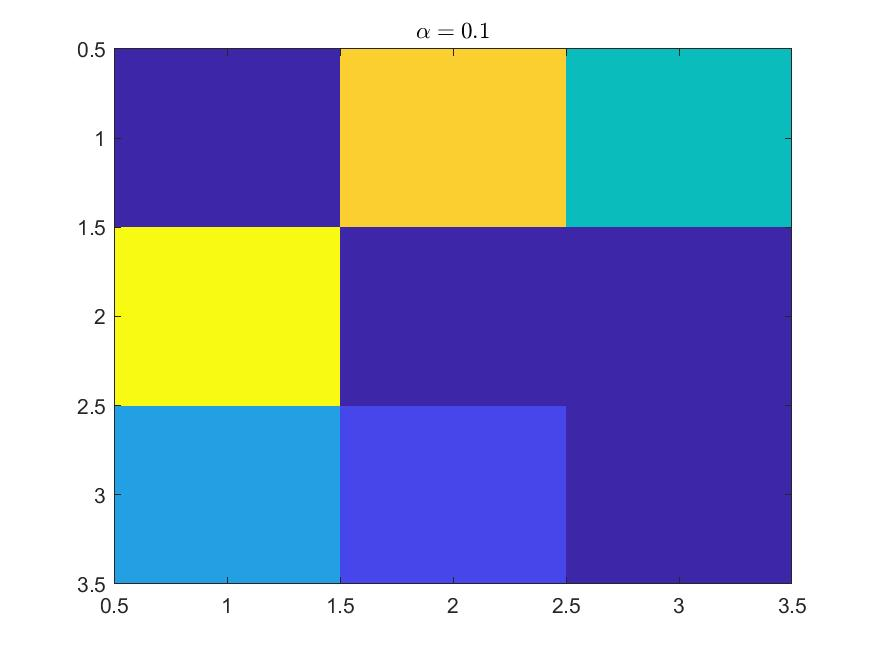
\includegraphics[width=.18\textwidth]{alpha1n3.jpg} & 
		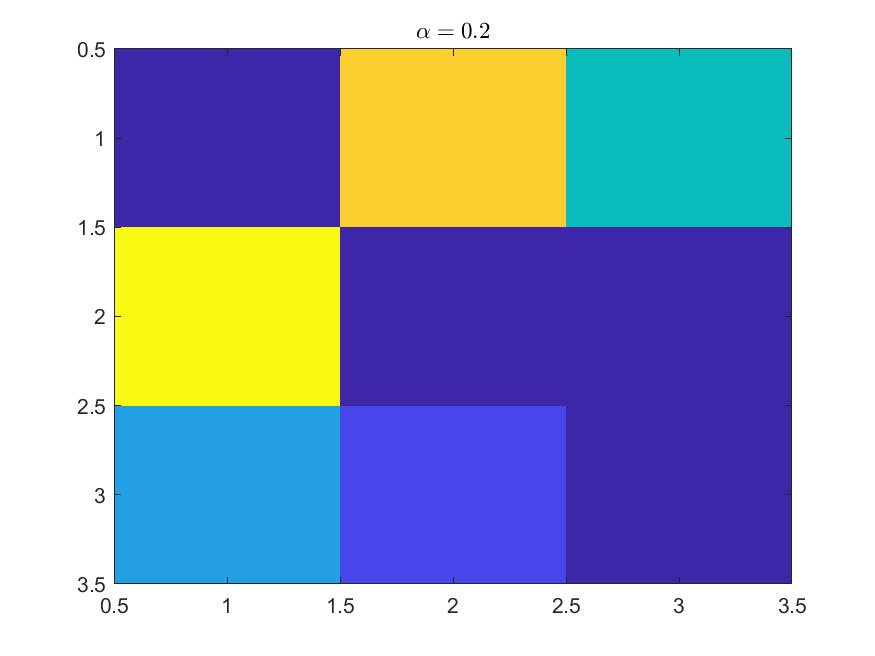
\includegraphics[width=.18\textwidth]{alpha2n3.jpg} & 
		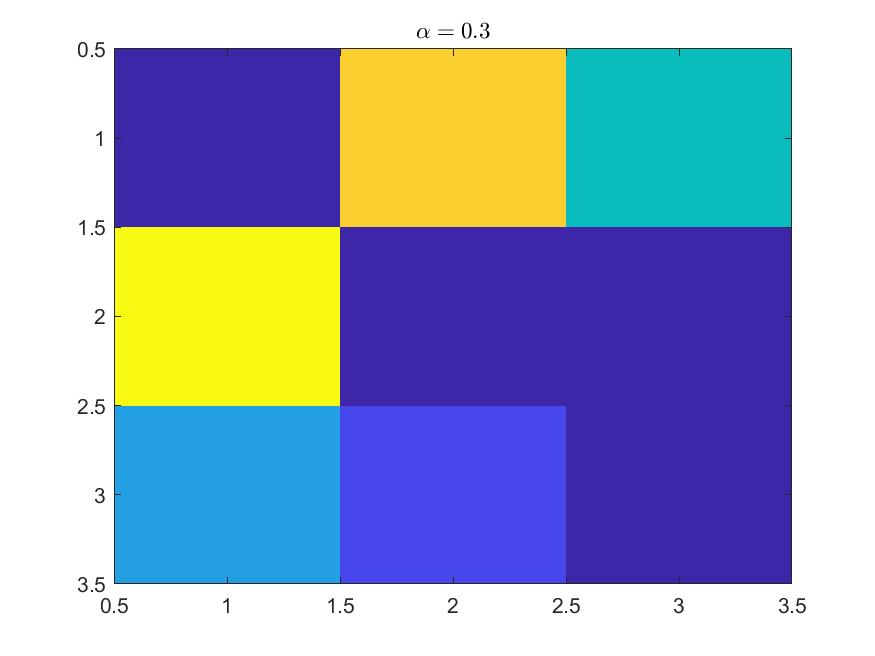
\includegraphics[width=.18\textwidth]{alpha3n3.jpg} & 
		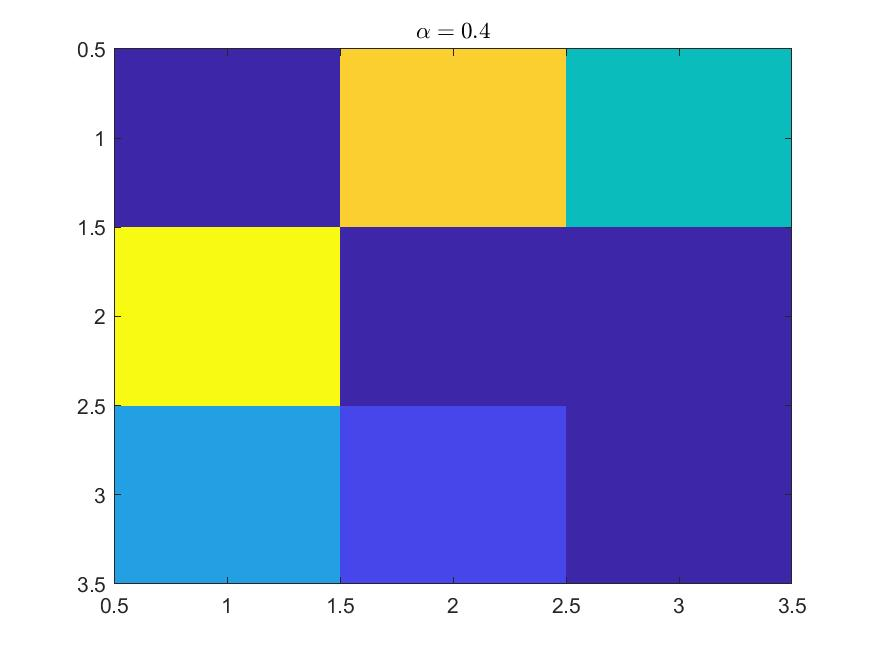
\includegraphics[width=.18\textwidth]{alpha4n3.jpg} & 
		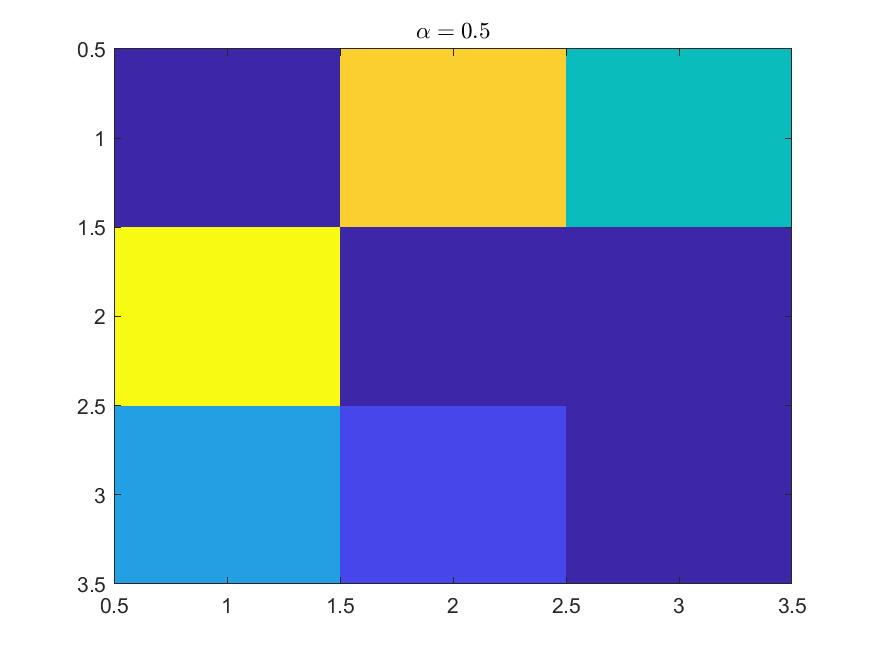
\includegraphics[width=.18\textwidth]{alpha5n3.jpg}\\
		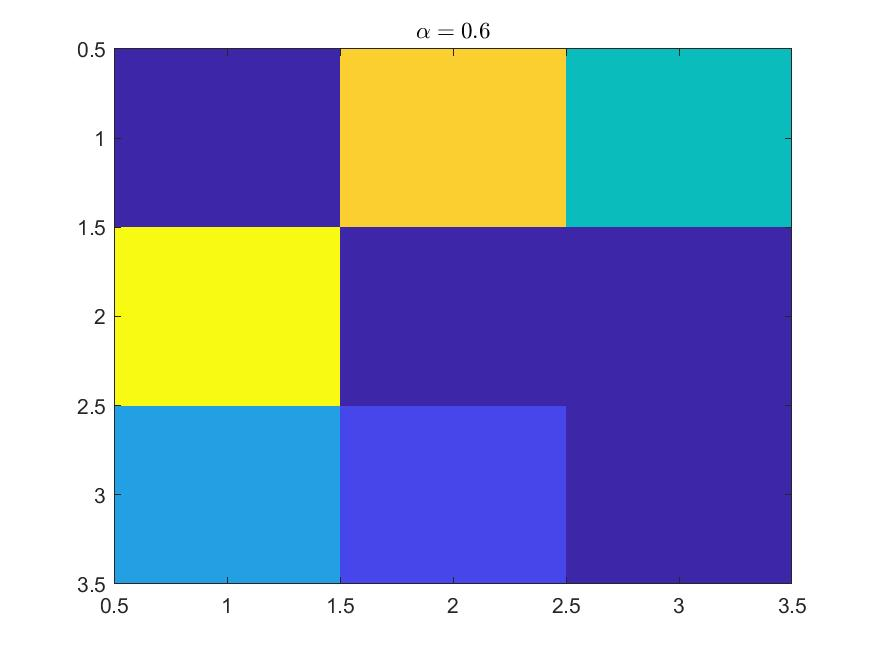
\includegraphics[width=.18\textwidth]{alpha6n3.jpg} & 
		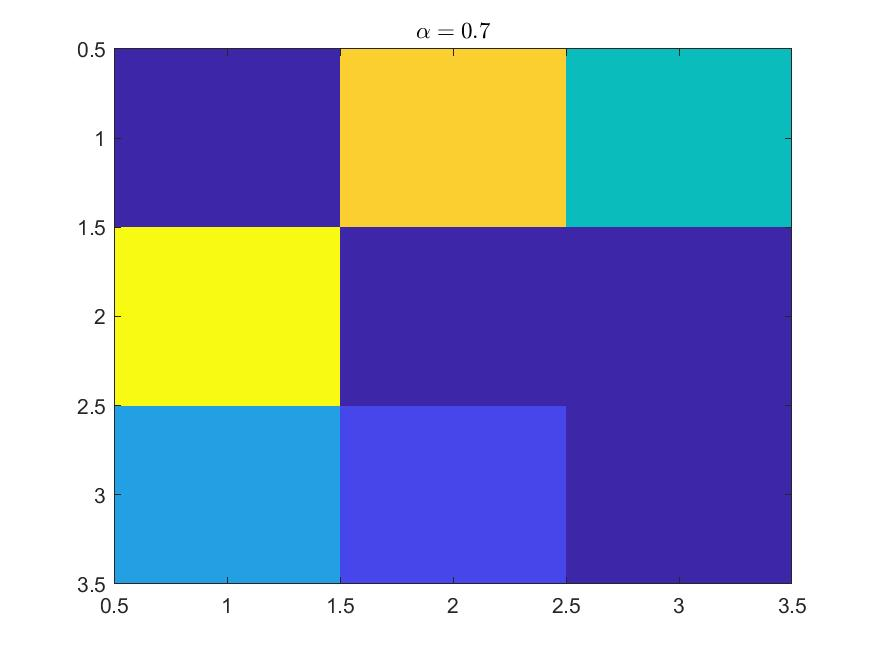
\includegraphics[width=.18\textwidth]{alpha7n3.jpg} &
		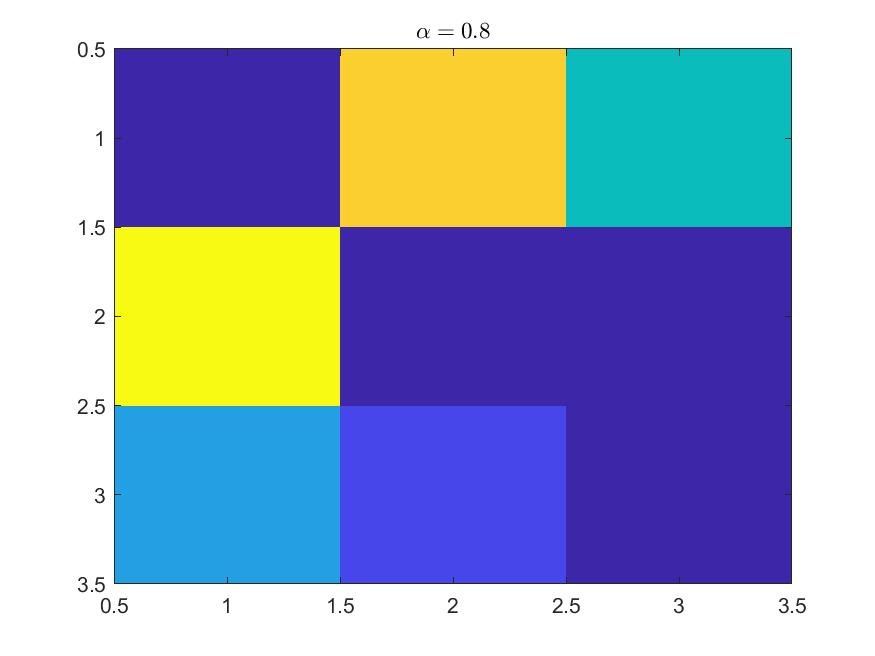
\includegraphics[width=.18\textwidth]{alpha8n3.jpg} & 
		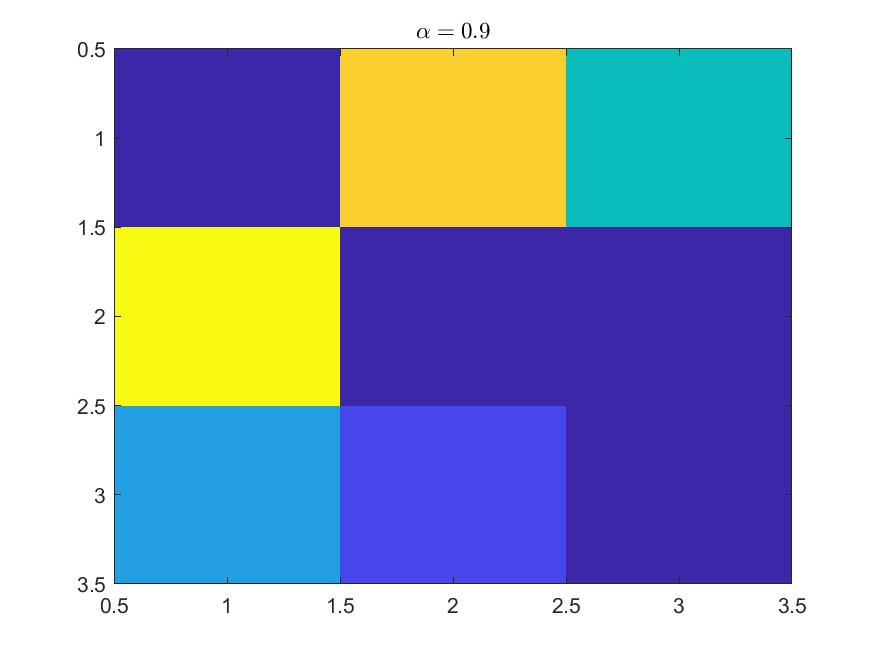
\includegraphics[width=.18\textwidth]{alpha9n3.jpg} & 
		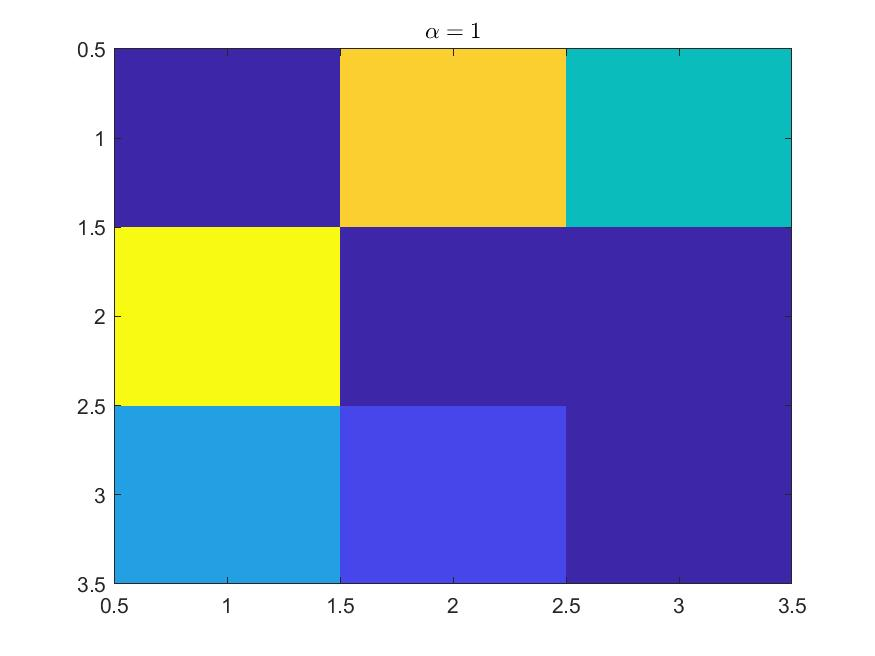
\includegraphics[width=.18\textwidth]{alpha10n3.jpg}
	\end{tabular}
	\caption{$n=3$, 不同松弛因子}
	\label{alphan3figure}
\end{figure}

\begin{figure}[htbp]
	\renewcommand{\captionfont}{\small}
	\centering
	\begin{tabular}{@{}ccccc@{}}
		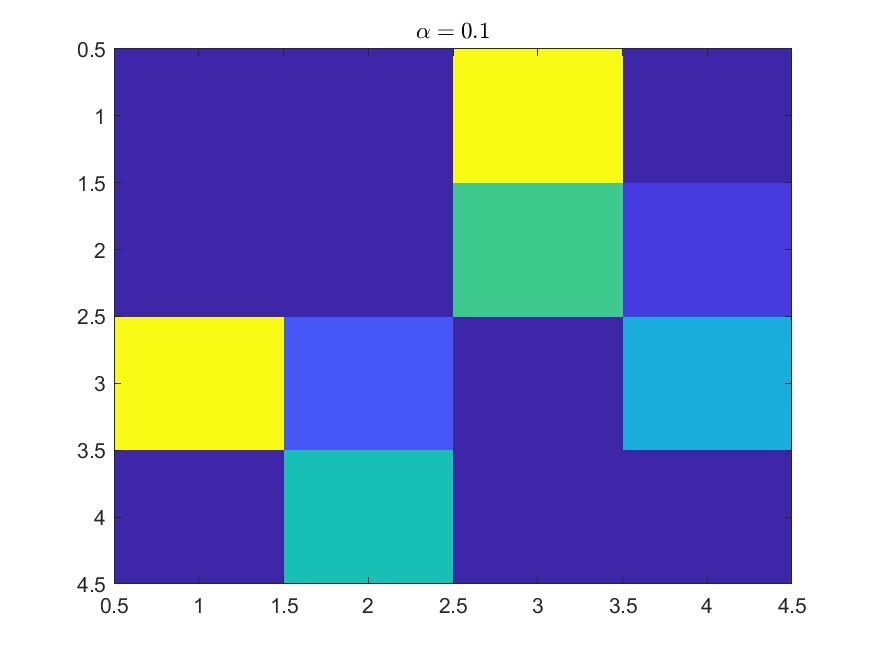
\includegraphics[width=.18\textwidth]{alpha1n4.jpg} & 
		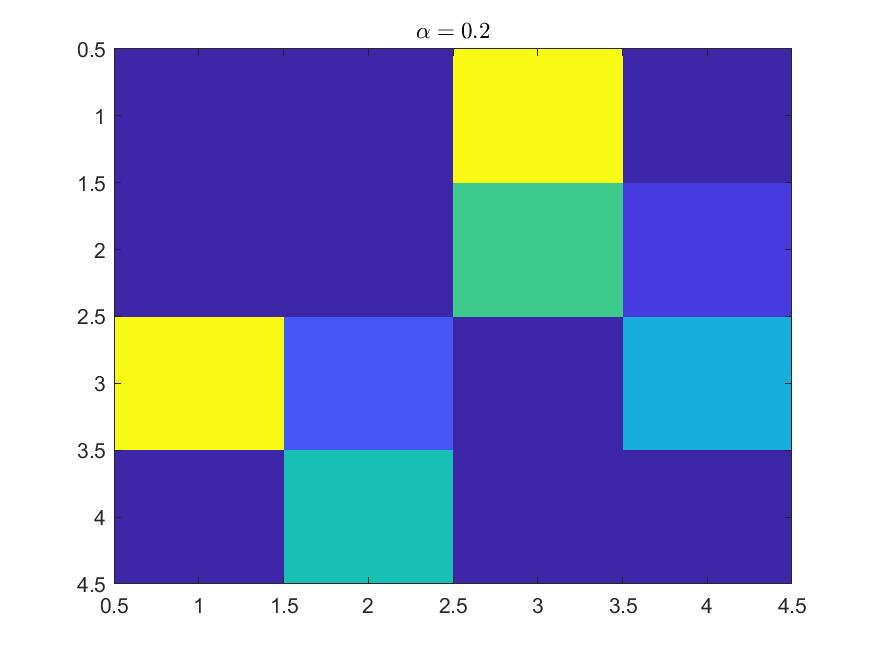
\includegraphics[width=.18\textwidth]{alpha2n4.jpg} & 
		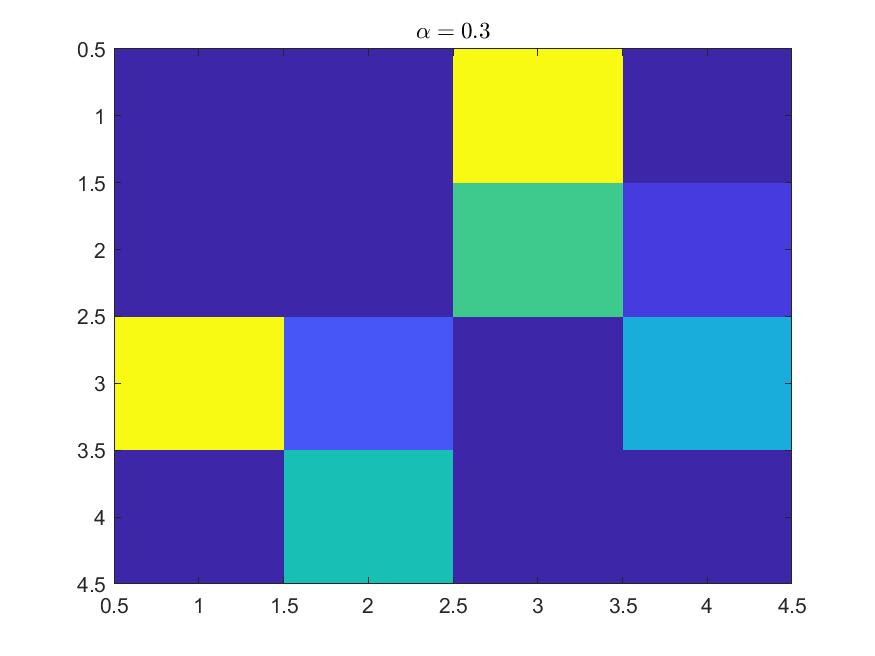
\includegraphics[width=.18\textwidth]{alpha3n4.jpg} & 
		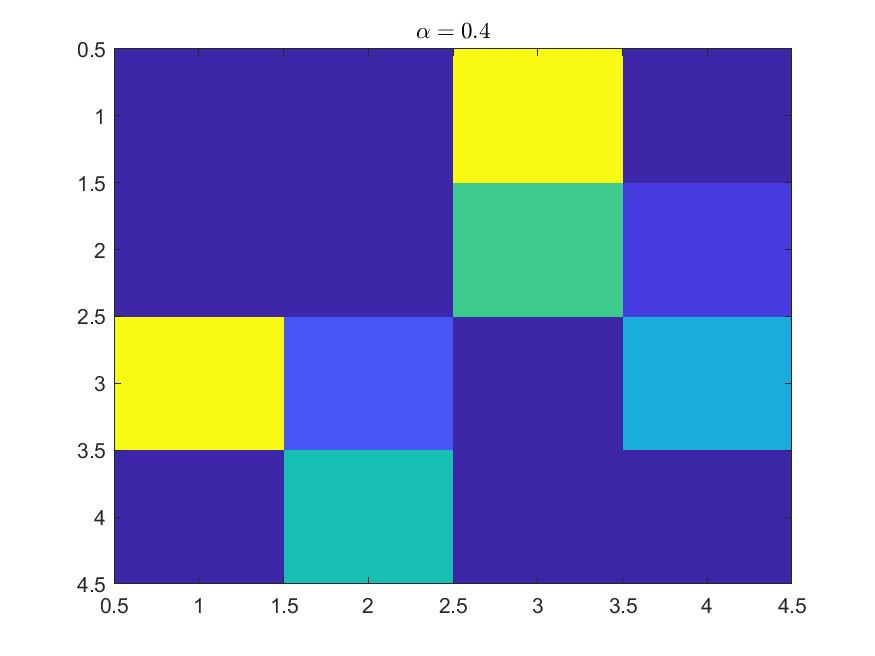
\includegraphics[width=.18\textwidth]{alpha4n4.jpg} & 
		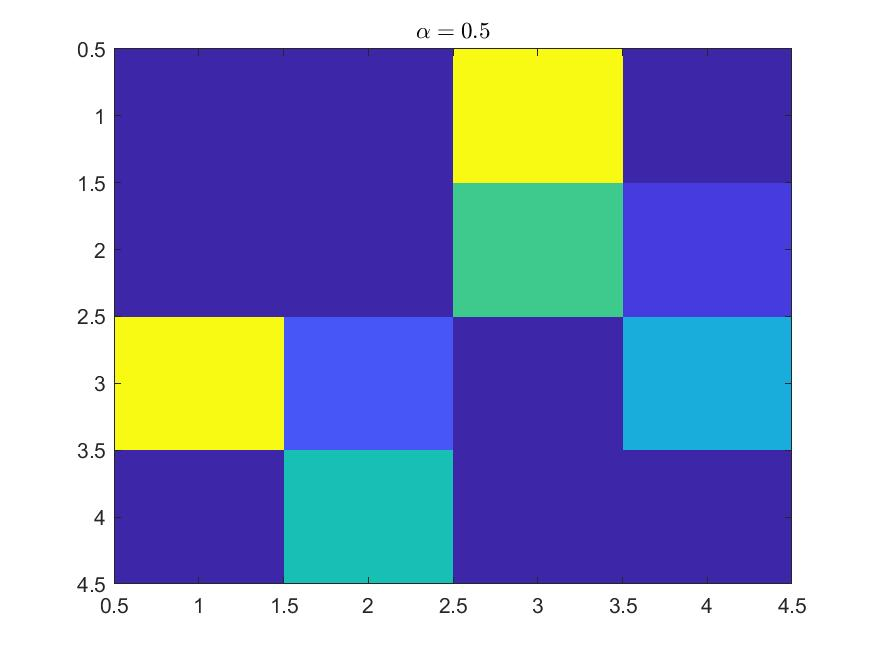
\includegraphics[width=.18\textwidth]{alpha5n4.jpg}\\
		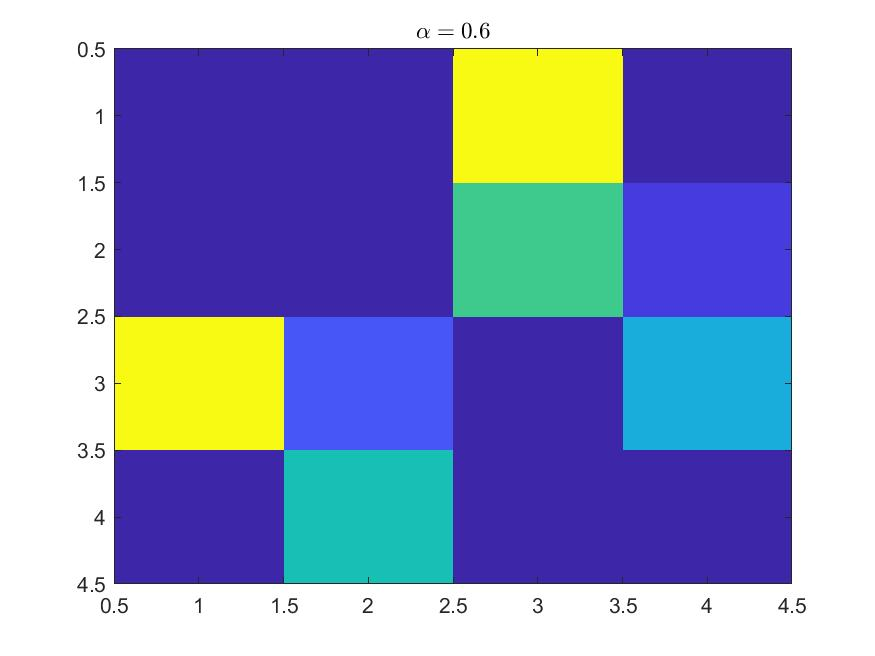
\includegraphics[width=.18\textwidth]{alpha6n4.jpg} & 
		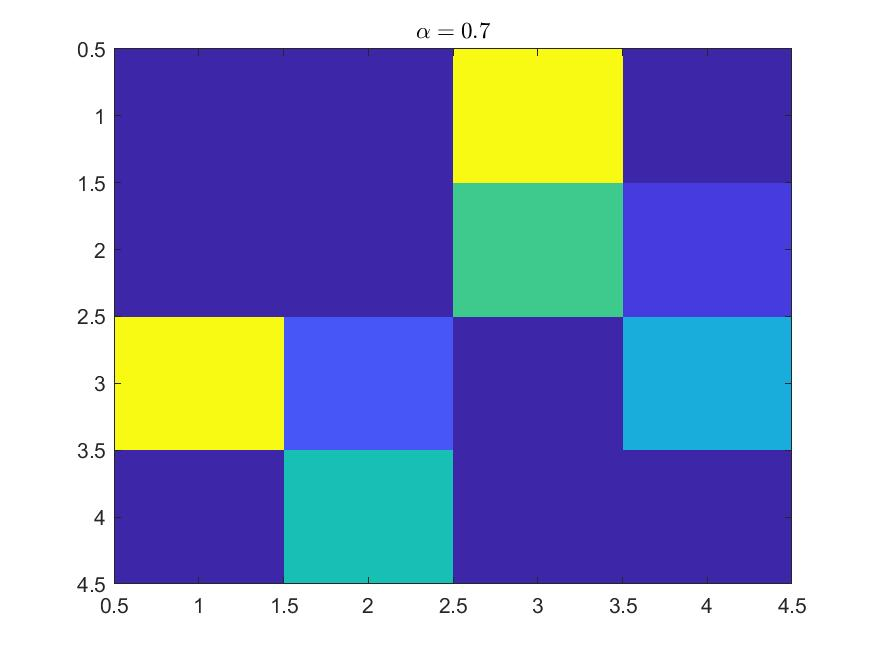
\includegraphics[width=.18\textwidth]{alpha7n4.jpg} &
		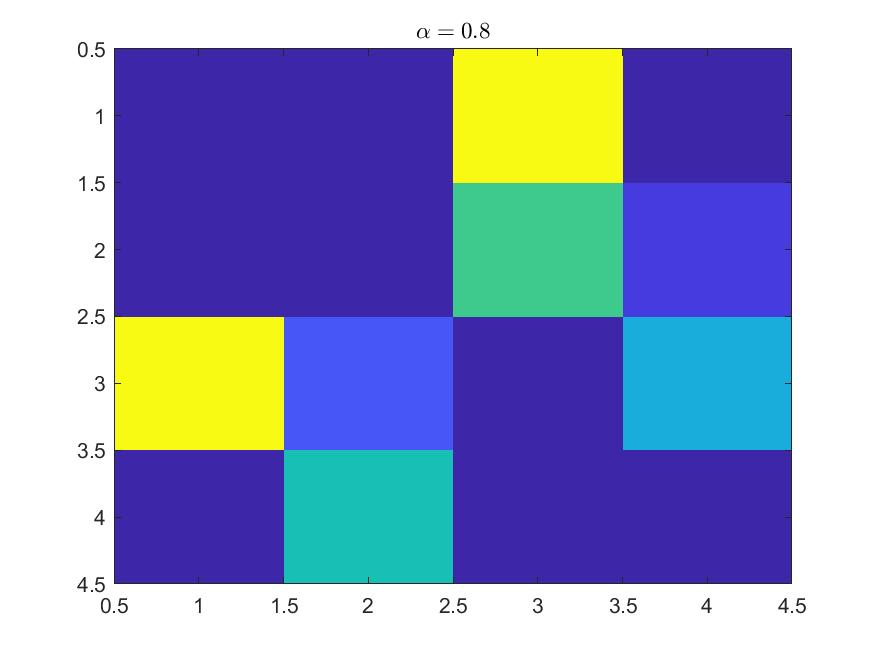
\includegraphics[width=.18\textwidth]{alpha8n4.jpg} & 
		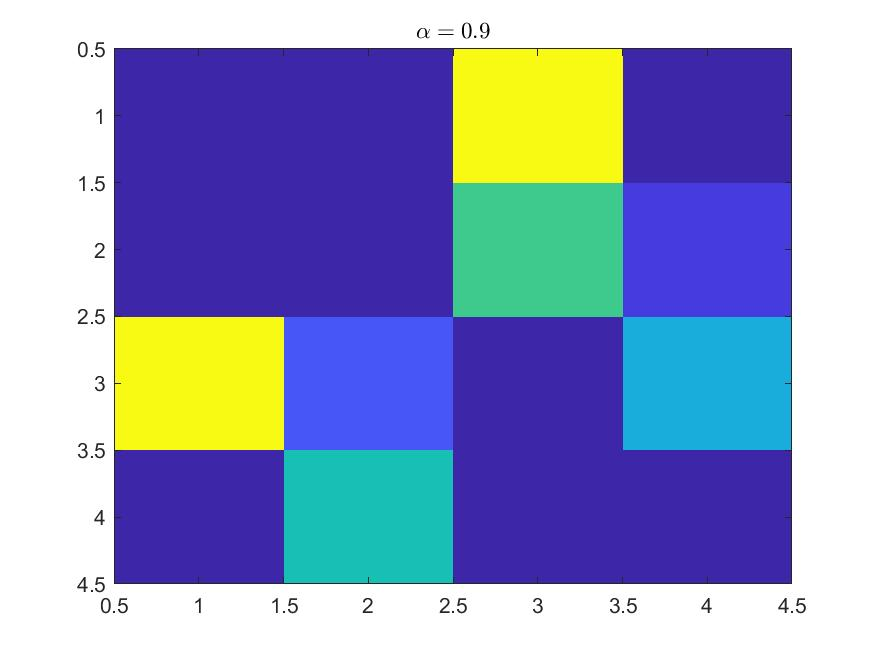
\includegraphics[width=.18\textwidth]{alpha9n4.jpg} & 
		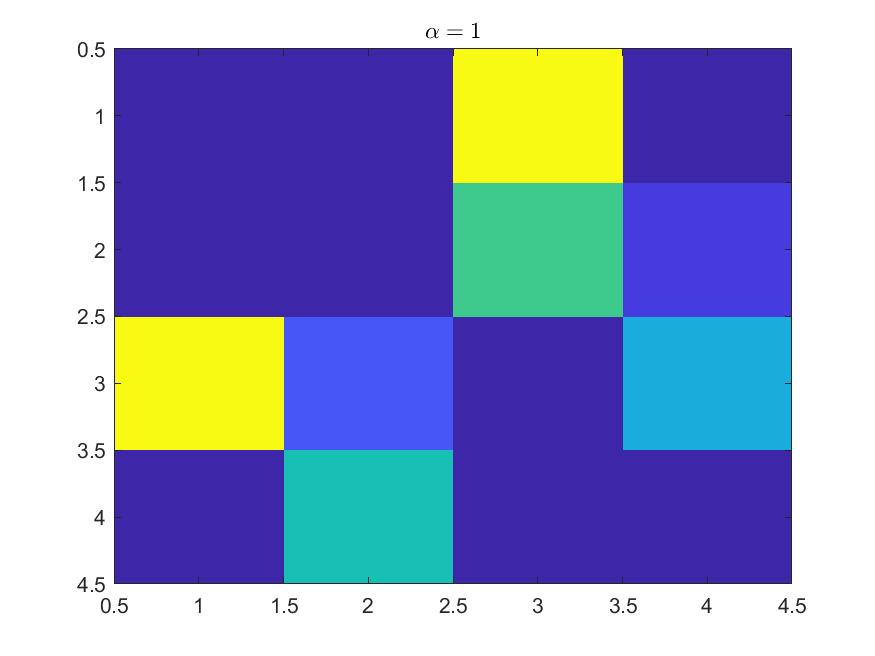
\includegraphics[width=.18\textwidth]{alpha10n4.jpg}
	\end{tabular}
	\caption{$n=4$, 不同松弛因子}
	\label{alphan4figure}
\end{figure}

\begin{figure}[htbp]
	\renewcommand{\captionfont}{\small}
	\centering
	\begin{tabular}{@{}ccccc@{}}
		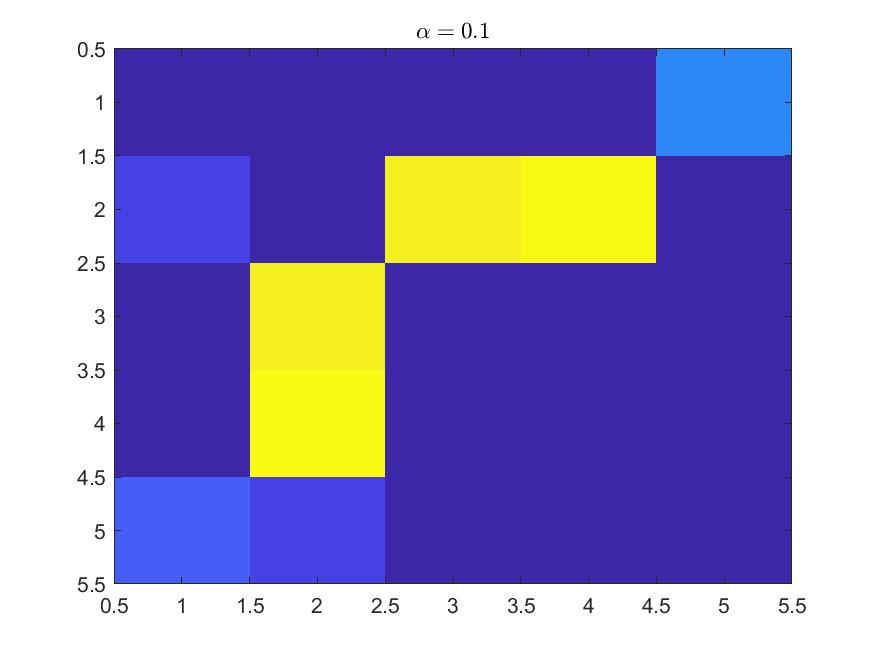
\includegraphics[width=.18\textwidth]{alpha1n5.jpg} & 
		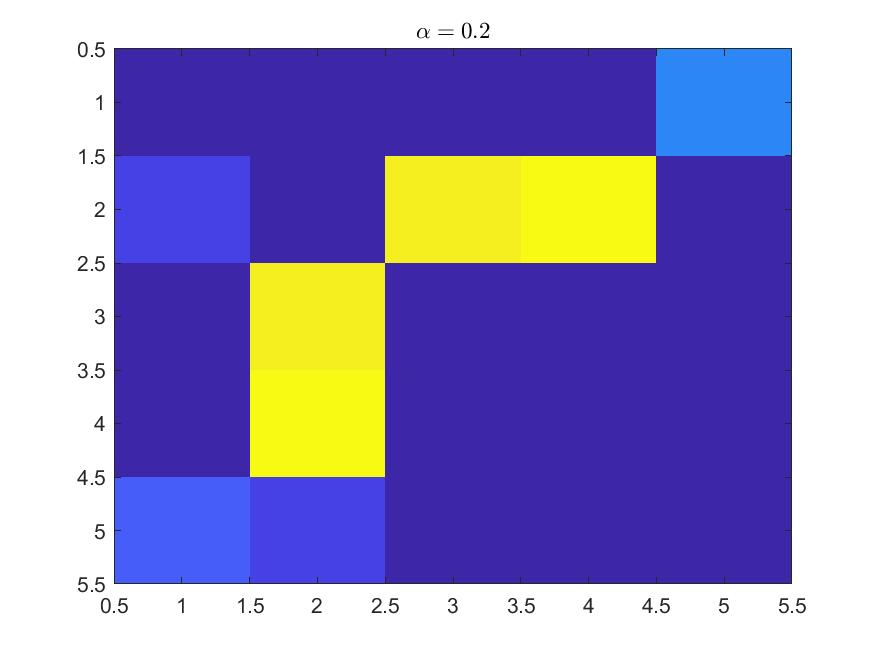
\includegraphics[width=.18\textwidth]{alpha2n5.jpg} & 
		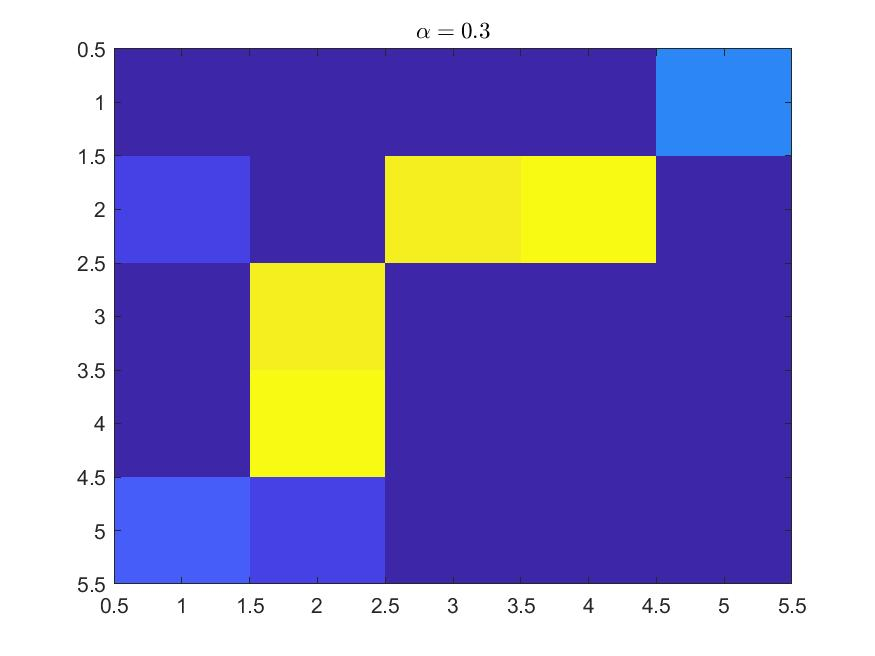
\includegraphics[width=.18\textwidth]{alpha3n5.jpg} & 
		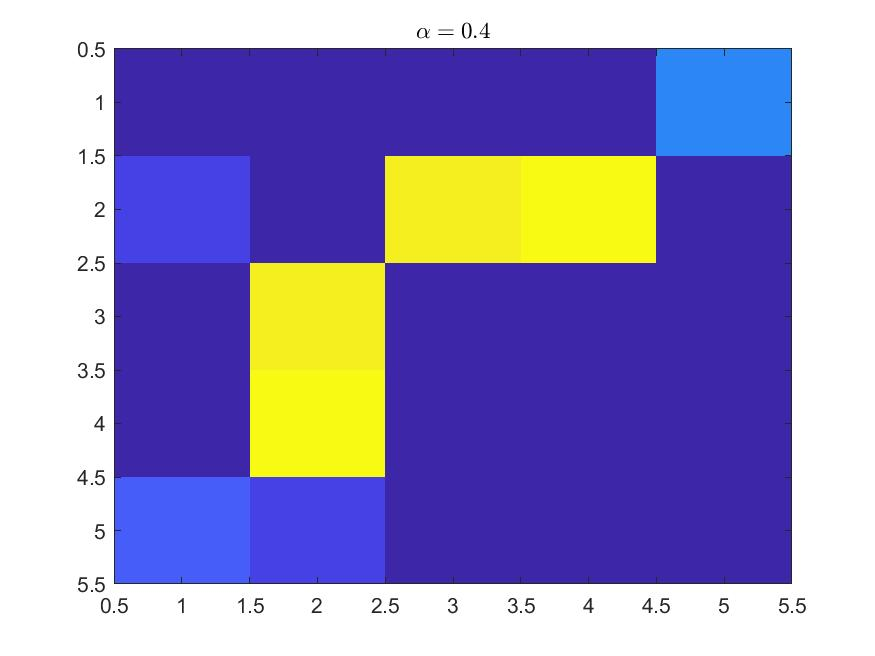
\includegraphics[width=.18\textwidth]{alpha4n5.jpg} & 
		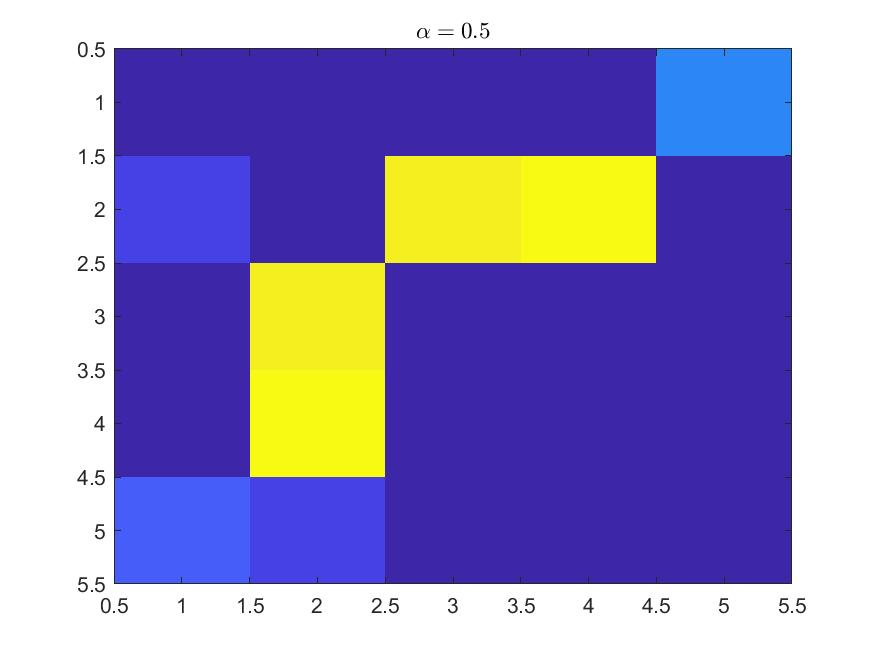
\includegraphics[width=.18\textwidth]{alpha5n5.jpg}\\
		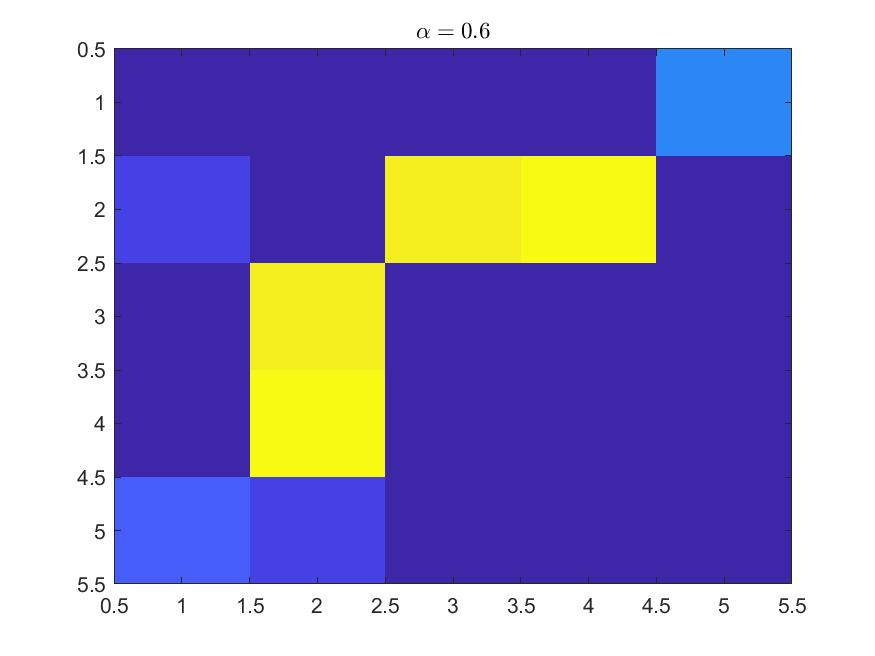
\includegraphics[width=.18\textwidth]{alpha6n5.jpg} & 
		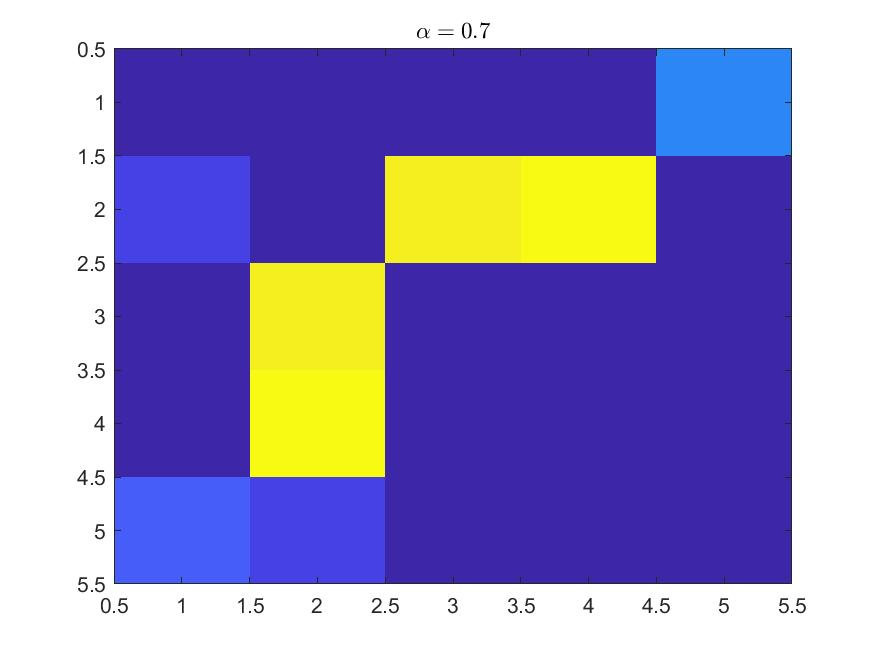
\includegraphics[width=.18\textwidth]{alpha7n5.jpg} &
		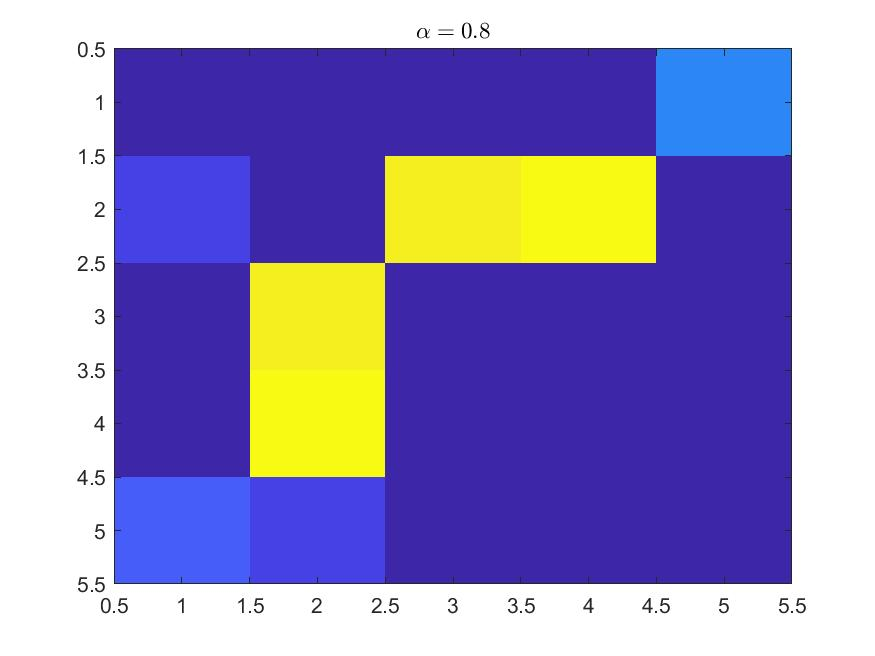
\includegraphics[width=.18\textwidth]{alpha8n5.jpg} & 
		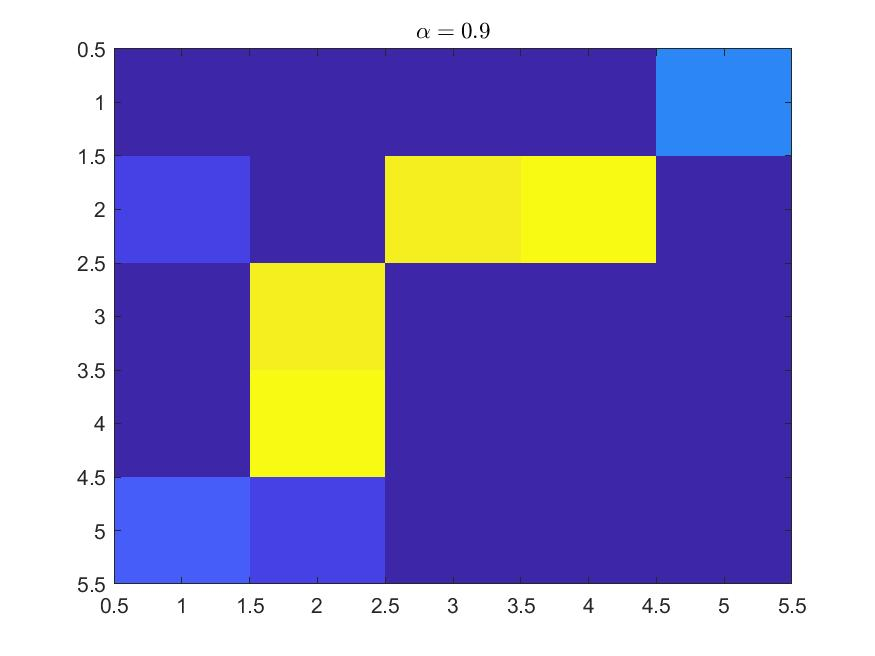
\includegraphics[width=.18\textwidth]{alpha9n5.jpg} & 
		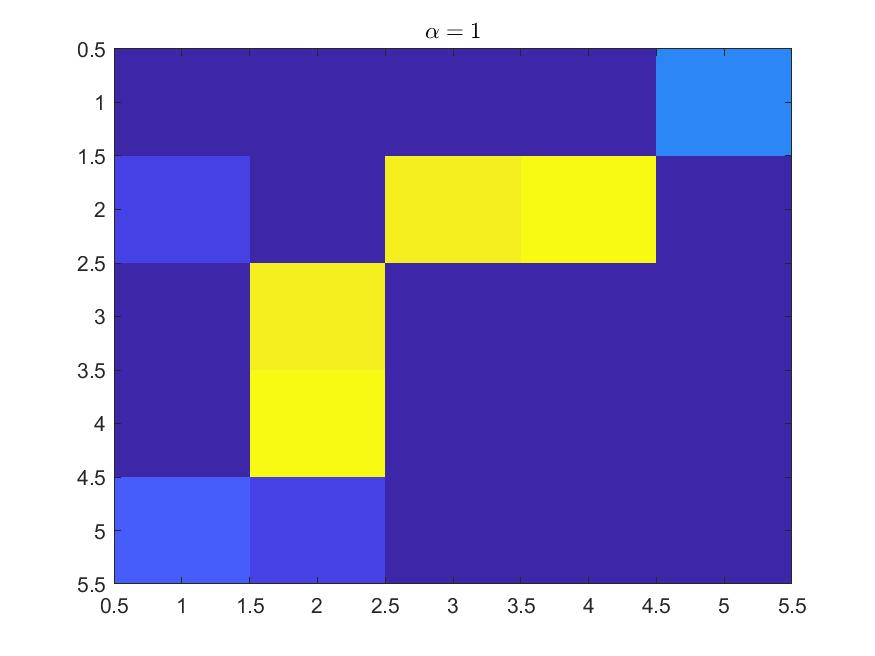
\includegraphics[width=.18\textwidth]{alpha10n5.jpg}
	\end{tabular}
	\caption{$n=5$, 不同松弛因子}
	\label{alphan5figure}
\end{figure}

\begin{figure}[htbp]
	\renewcommand{\captionfont}{\small}
	\centering
	\begin{tabular}{@{}ccccc@{}}
		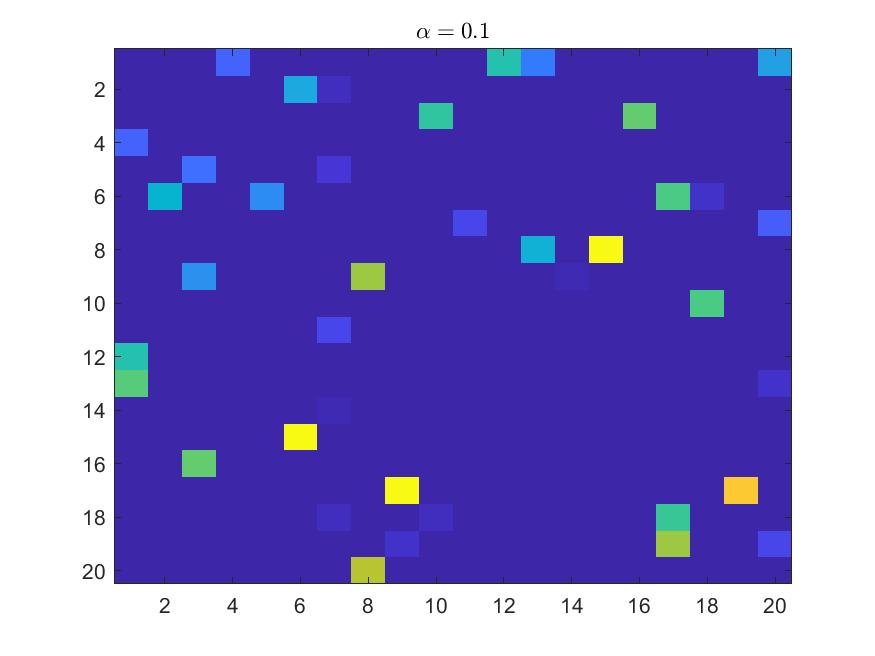
\includegraphics[width=.18\textwidth]{alpha1n20.jpg} & 
		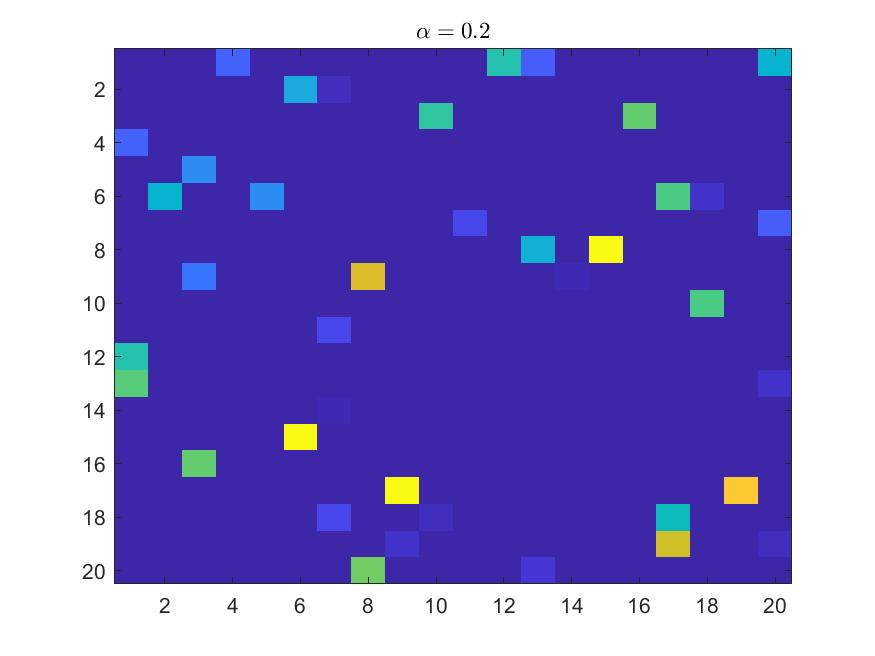
\includegraphics[width=.18\textwidth]{alpha2n20.jpg} & 
		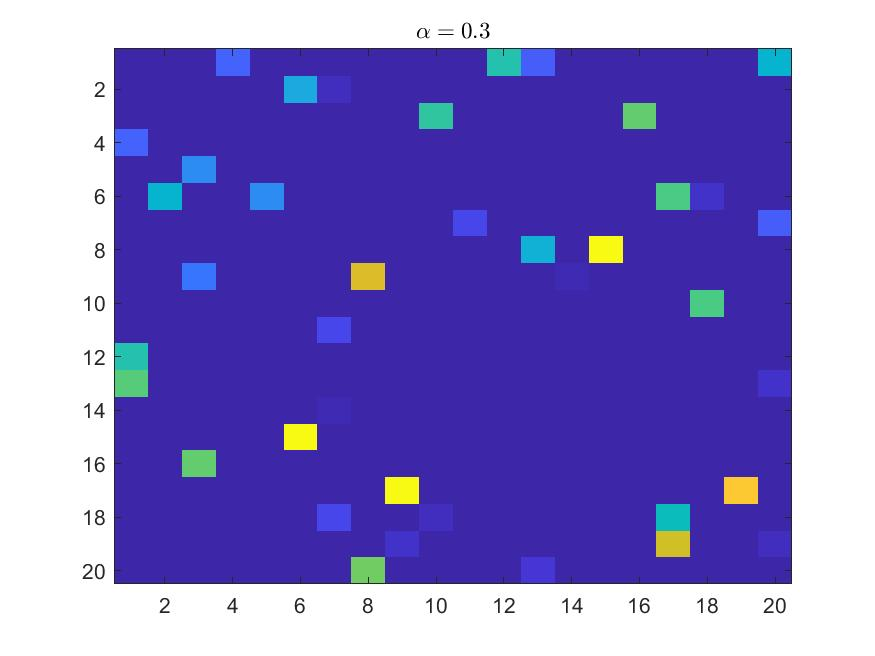
\includegraphics[width=.18\textwidth]{alpha3n20.jpg} & 
		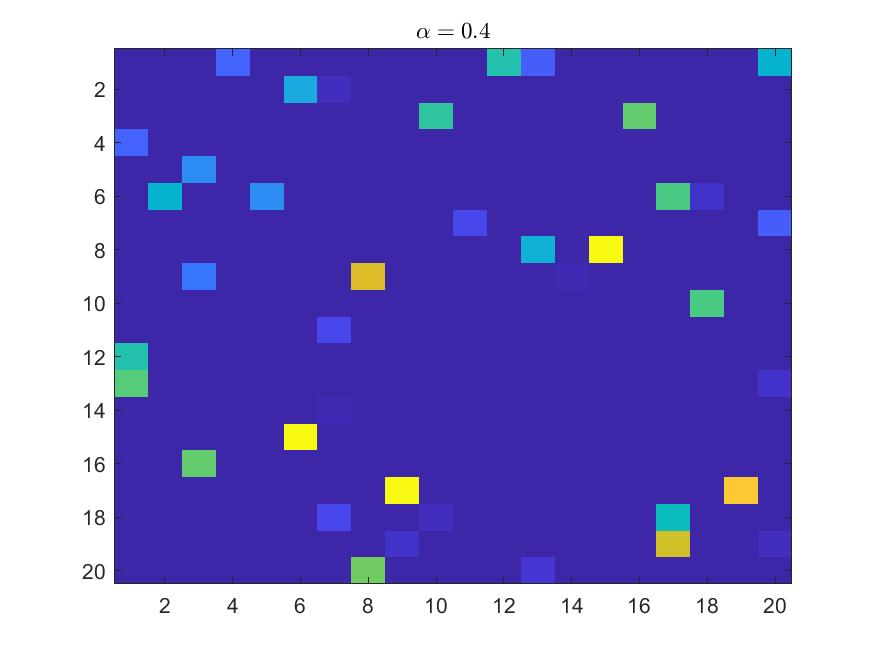
\includegraphics[width=.18\textwidth]{alpha4n20.jpg} & 
		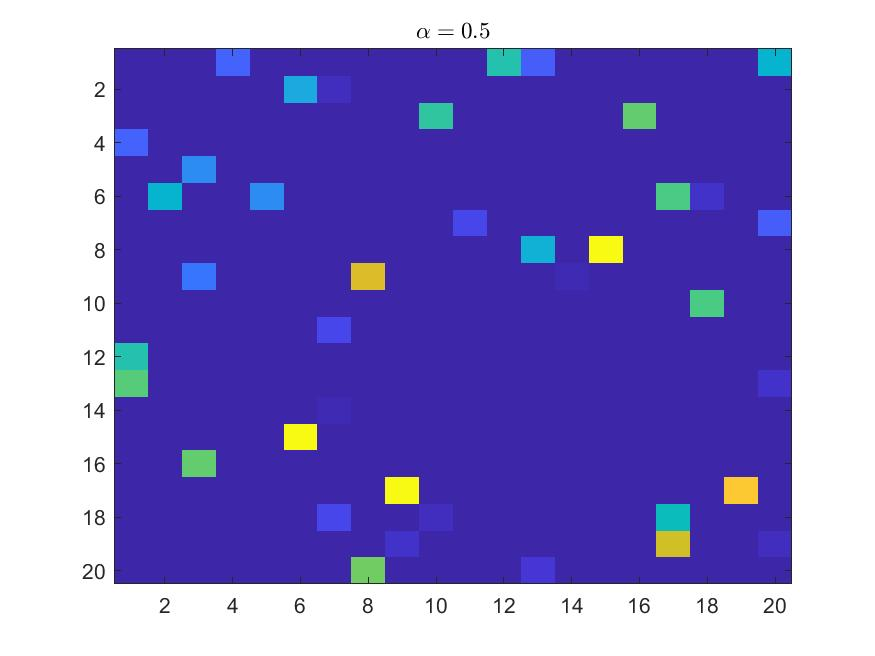
\includegraphics[width=.18\textwidth]{alpha5n20.jpg}\\
		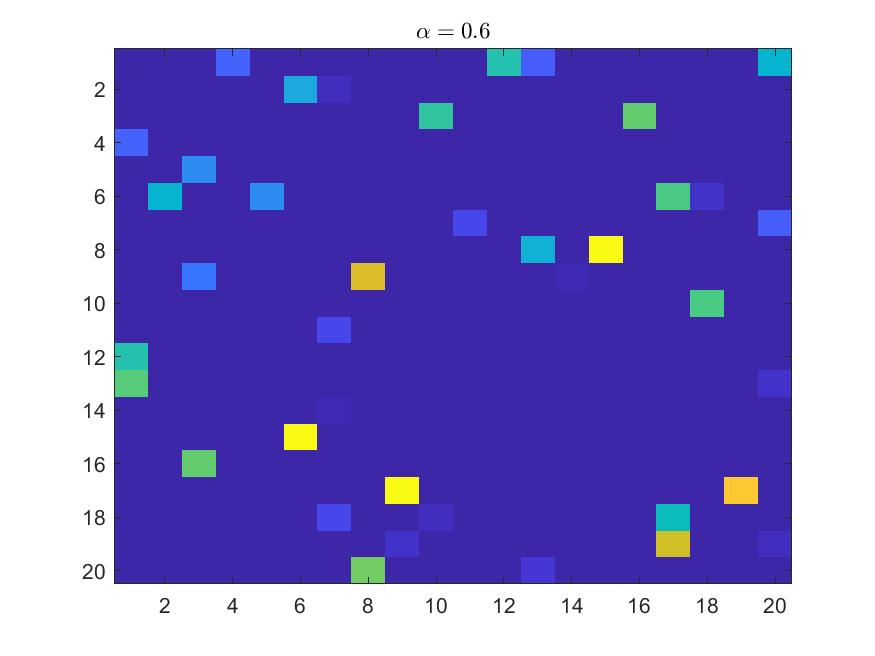
\includegraphics[width=.18\textwidth]{alpha6n20.jpg} & 
		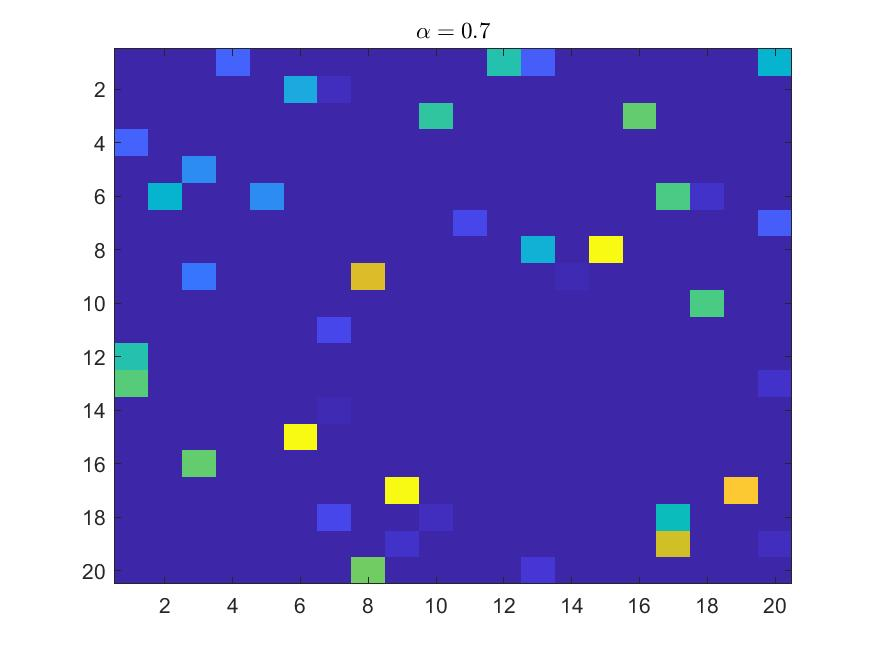
\includegraphics[width=.18\textwidth]{alpha7n20.jpg} &
		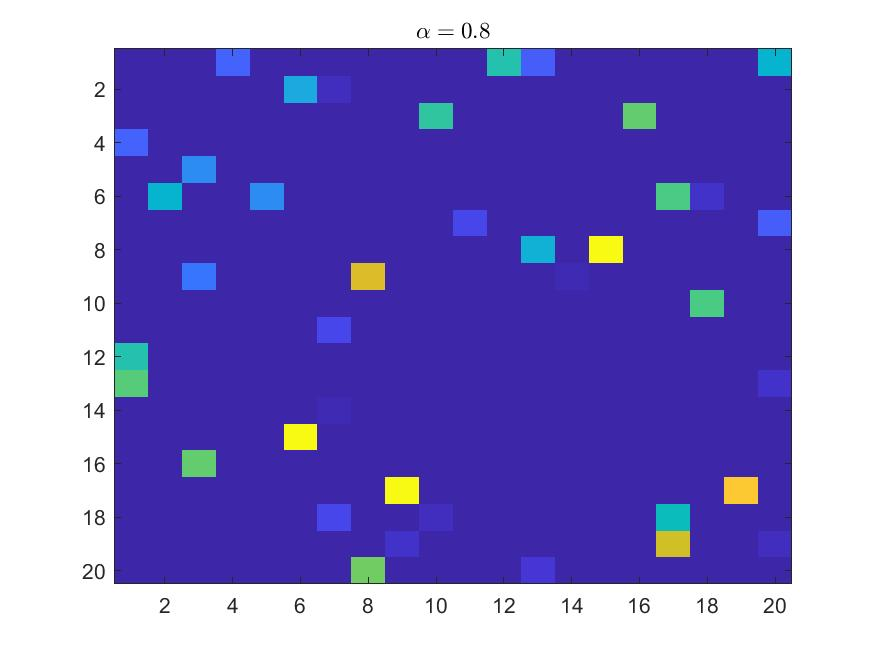
\includegraphics[width=.18\textwidth]{alpha8n20.jpg} & 
		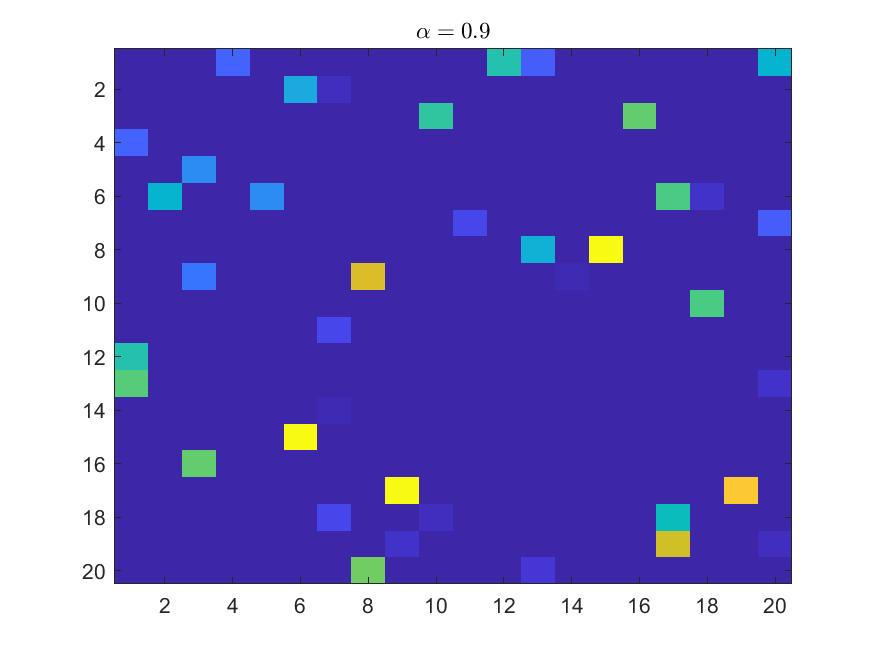
\includegraphics[width=.18\textwidth]{alpha9n20.jpg} & 
		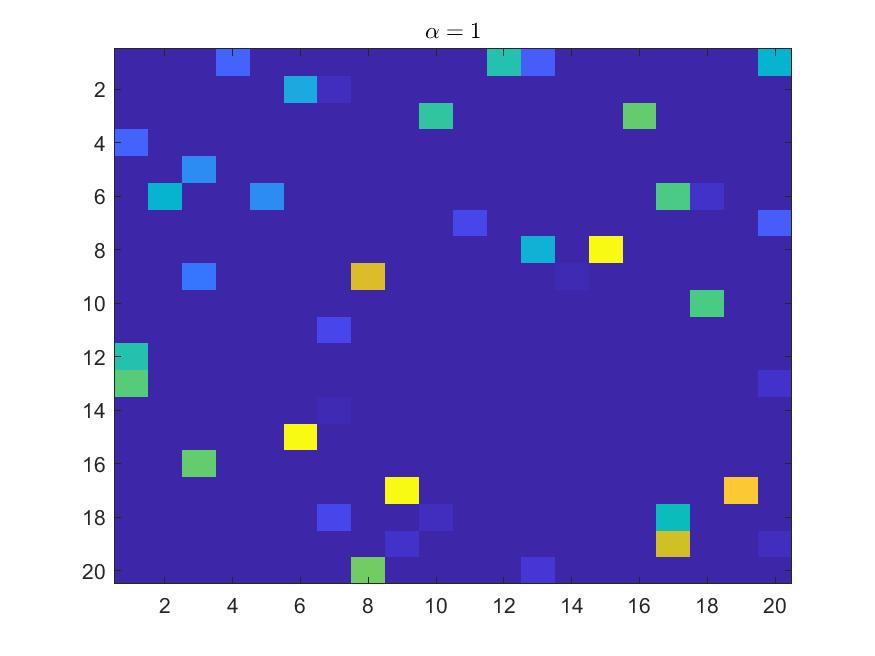
\includegraphics[width=.18\textwidth]{alpha10n20.jpg}
	\end{tabular}
	\caption{$n=20$, 不同松弛因子}
	\label{alphan20figure}
\end{figure}

\begin{figure}[htbp]
	\renewcommand{\captionfont}{\small}
	\centering
	\begin{tabular}{@{}ccccc@{}}
		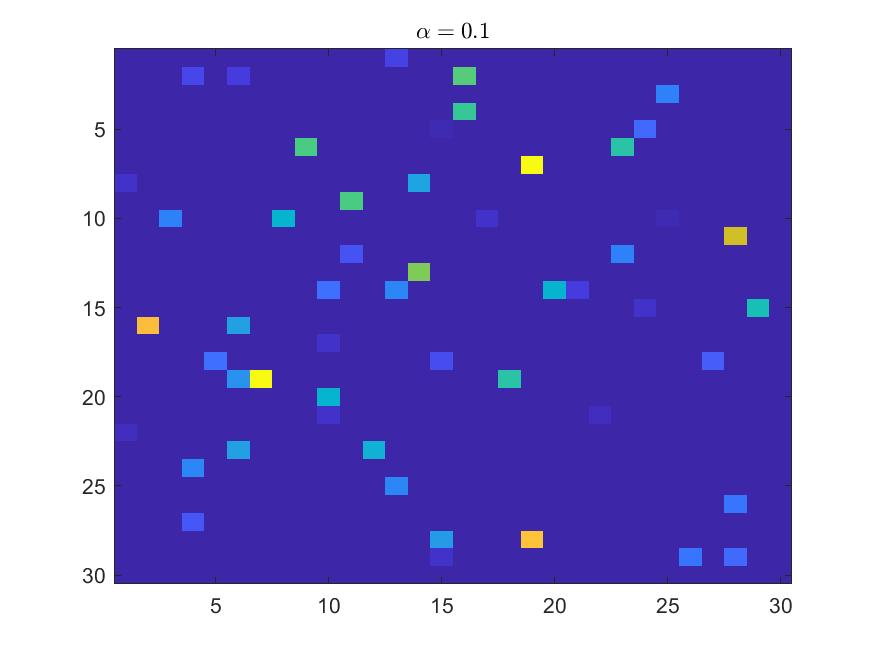
\includegraphics[width=.18\textwidth]{alpha1n30.jpg} & 
		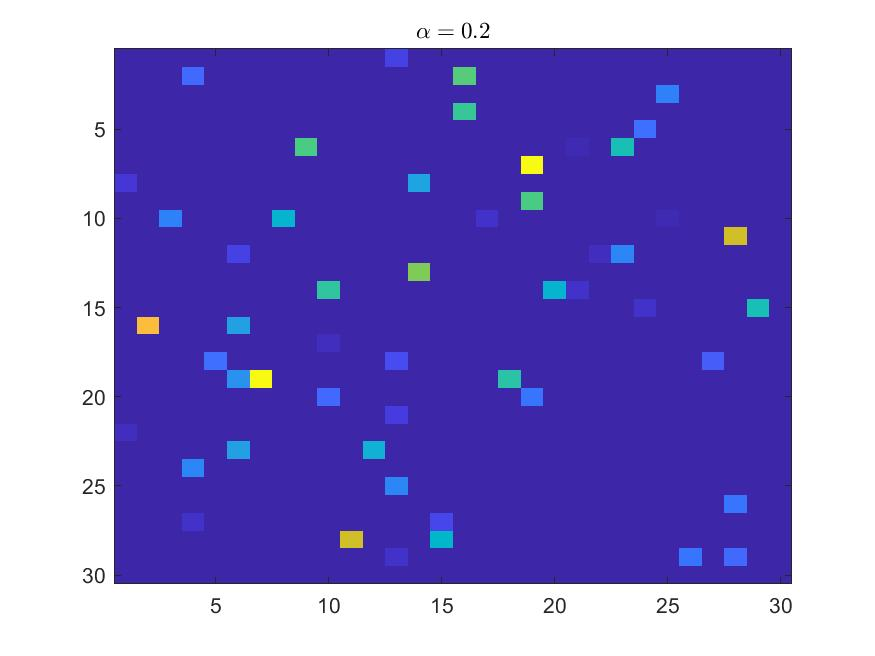
\includegraphics[width=.18\textwidth]{alpha2n30.jpg} & 
		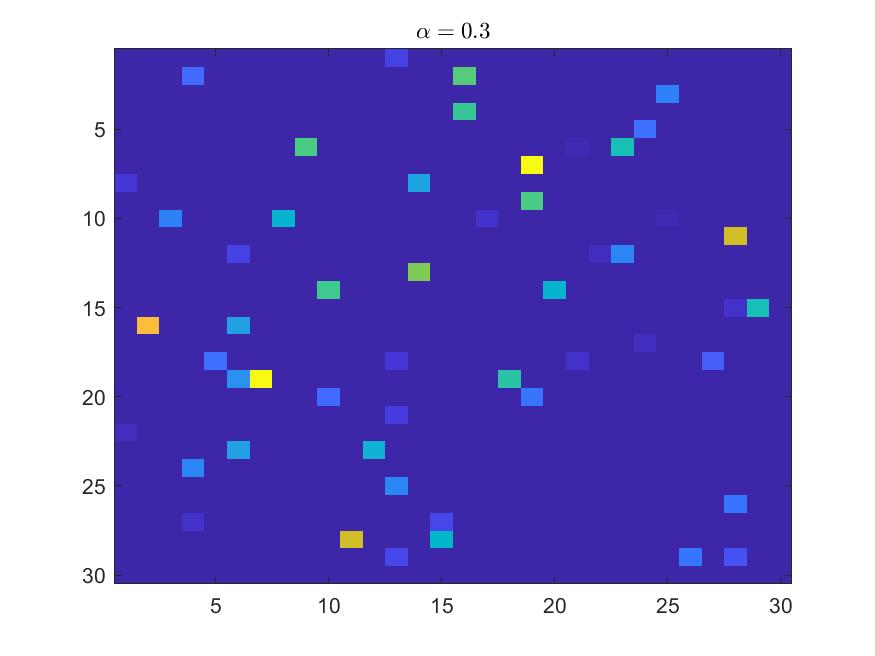
\includegraphics[width=.18\textwidth]{alpha3n30.jpg} & 
		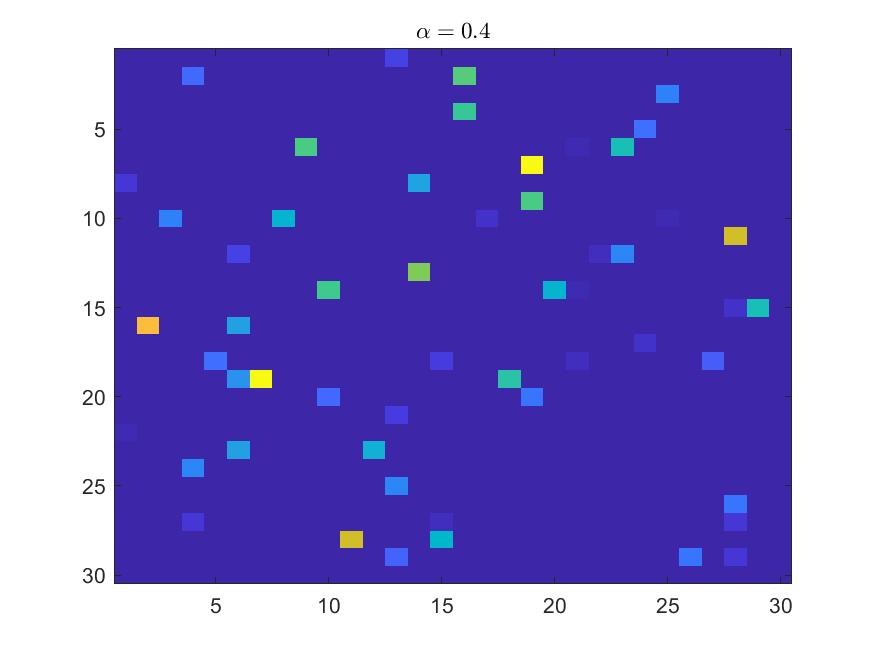
\includegraphics[width=.18\textwidth]{alpha4n30.jpg} & 
		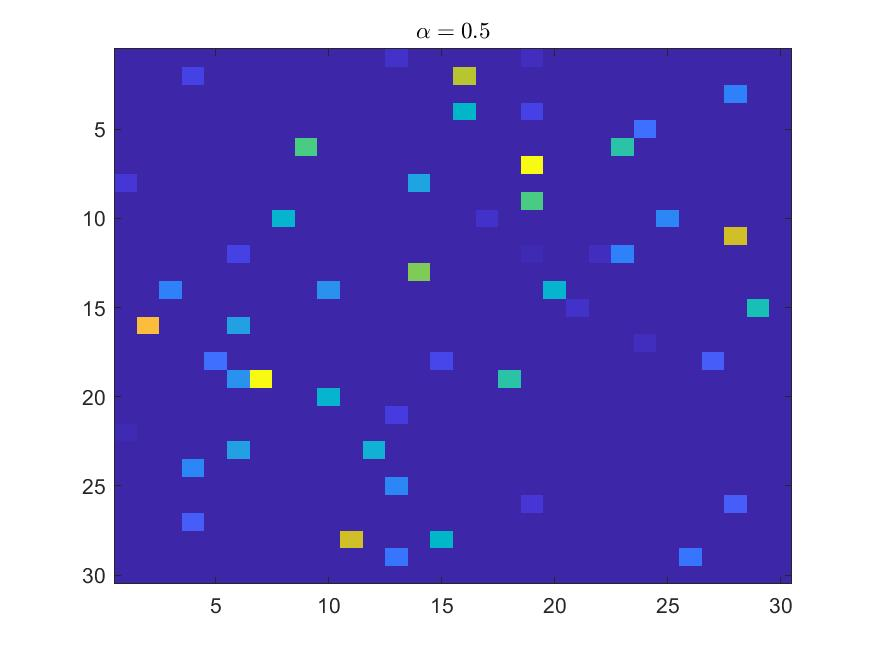
\includegraphics[width=.18\textwidth]{alpha5n30.jpg}\\
		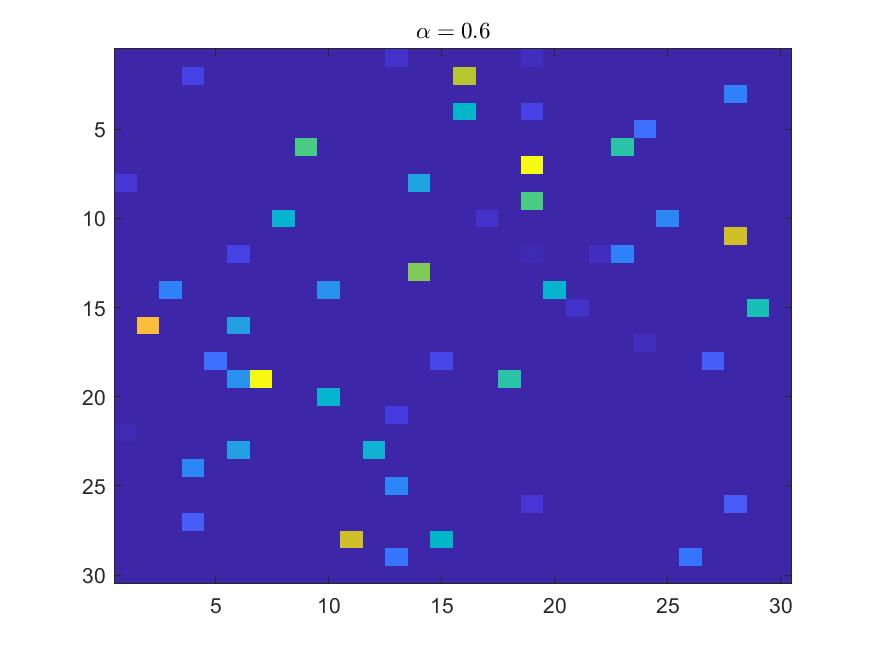
\includegraphics[width=.18\textwidth]{alpha6n30.jpg} & 
		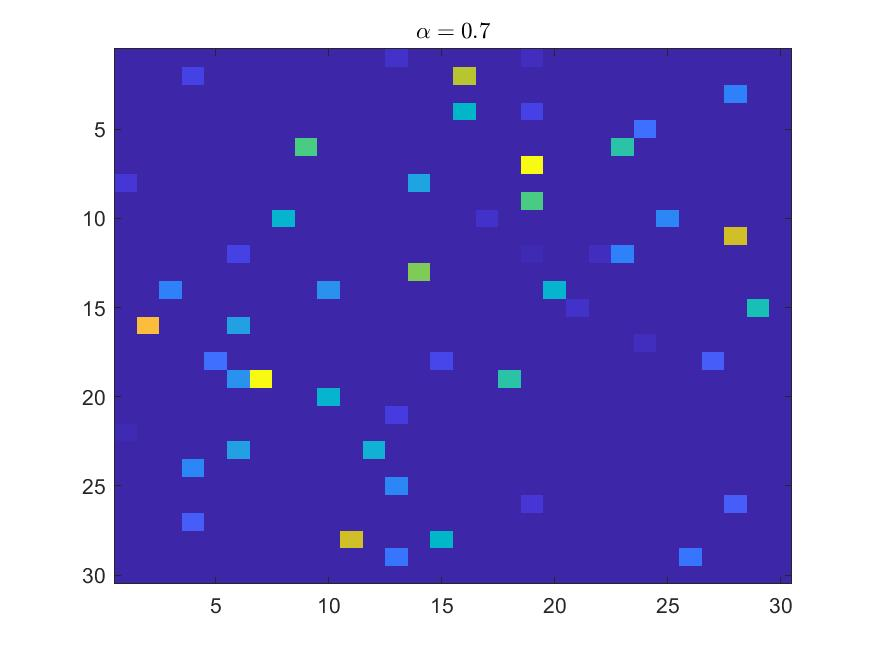
\includegraphics[width=.18\textwidth]{alpha7n30.jpg} &
		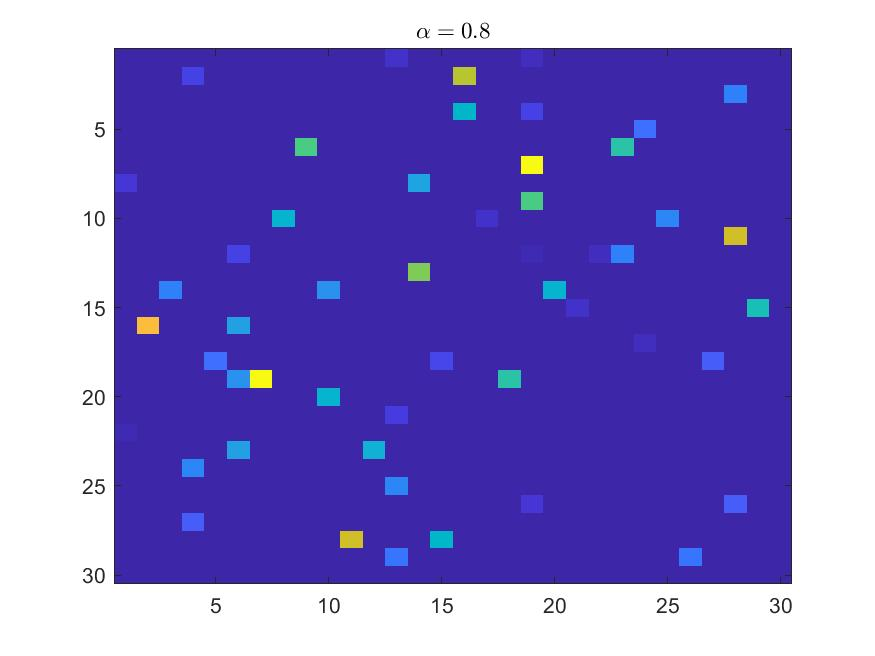
\includegraphics[width=.18\textwidth]{alpha8n30.jpg} & 
		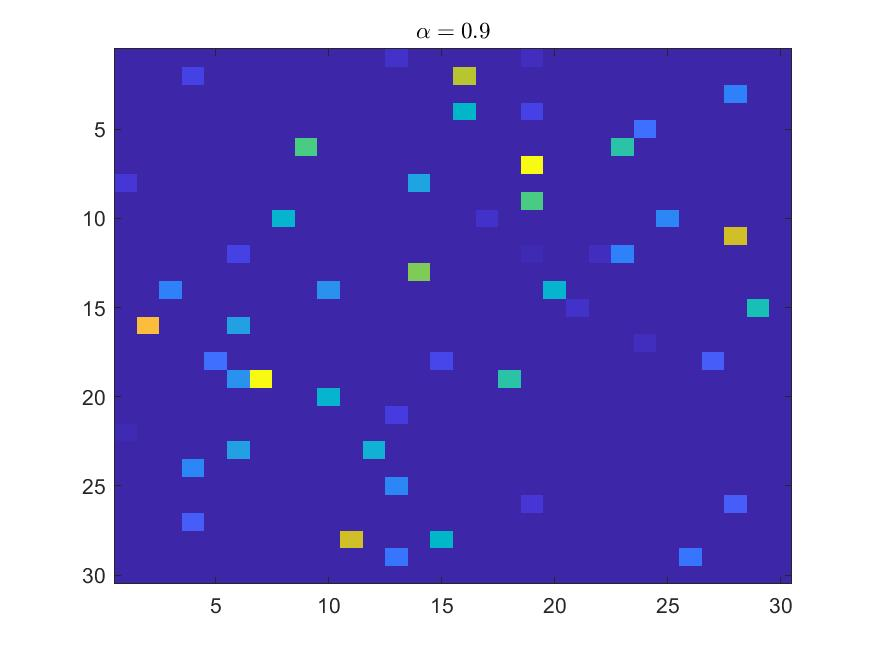
\includegraphics[width=.18\textwidth]{alpha9n30.jpg} & 
		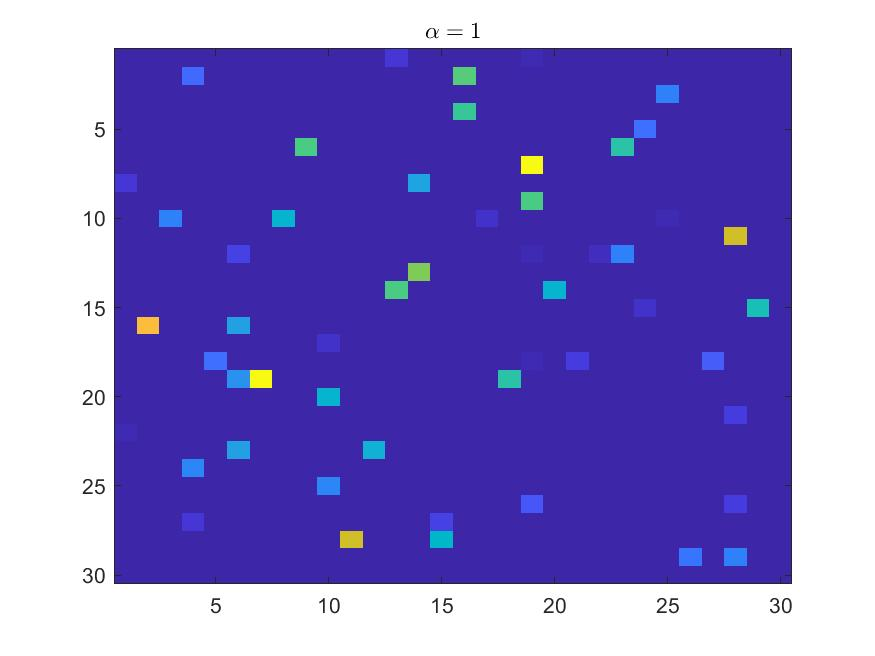
\includegraphics[width=.18\textwidth]{alpha10n30.jpg}
	\end{tabular}
	\caption{$n=30$, 不同松弛因子}
	\label{alphan30figure}
\end{figure}

\begin{figure}[htbp]
	\renewcommand{\captionfont}{\small}
	\centering
	\begin{tabular}{@{}ccccc@{}}
		\includegraphics[width=.18\textwidth]{alpha1n40.jpg} & 
		\includegraphics[width=.18\textwidth]{alpha2n40.jpg} & 
		\includegraphics[width=.18\textwidth]{alpha3n40.jpg} & 
		\includegraphics[width=.18\textwidth]{alpha4n40.jpg} & 
		\includegraphics[width=.18\textwidth]{alpha5n40.jpg}\\
		\includegraphics[width=.18\textwidth]{alpha6n40.jpg} & 
		\includegraphics[width=.18\textwidth]{alpha7n40.jpg} &
		\includegraphics[width=.18\textwidth]{alpha8n40.jpg} & 
		\includegraphics[width=.18\textwidth]{alpha9n40.jpg} & 
		\includegraphics[width=.18\textwidth]{alpha10n40.jpg}
	\end{tabular}
	\caption{$n=40$, 不同松弛因子}
	\label{alphan40figure}
\end{figure}
图中不同颜色代表了不同的取值, 颜色相近代表取值相近.
\par 典型的收敛曲线如图\ref{converge curve}所示. 
\begin{figure}[htbp]
	\renewcommand{\captionfont}{\small}
	\centering
	\subfigure[$\alpha=0.1,n=3$]{
	\begin{minipage}[b]{.31\linewidth}
		\includegraphics[width=\linewidth]{n3primalres.jpg}\vspace{4pt}
		\includegraphics[width=\linewidth]{n3dualres.jpg}\vspace{4pt}
		\includegraphics[width=\linewidth]{n3obj.jpg}
	\end{minipage}
	}
	\subfigure[$\alpha=0.2,n=4$]{
		\begin{minipage}[b]{.31\linewidth}
			\includegraphics[width=\linewidth]{n4primalres.jpg}\vspace{4pt}
			\includegraphics[width=\linewidth]{n4dualres.jpg}\vspace{4pt}
			\includegraphics[width=\linewidth]{n4obj.jpg}
		\end{minipage}
		}
	\subfigure[$\alpha=0.8,n=5$]{
		\begin{minipage}[b]{.31\linewidth}
			\includegraphics[width=\linewidth]{n5primalres.jpg}\vspace{4pt}
			\includegraphics[width=\linewidth]{n5dualres.jpg}\vspace{4pt}
			\includegraphics[width=\linewidth]{n5obj.jpg}
		\end{minipage}
		}
	\caption{收敛曲线}
	\label{converge curve}
\end{figure}
其中第一行为目标函数值, 第二行为KKT违反度, 第三行为增广拉格朗日函数值. 其中第二行的$y$轴数据以10为底. 从图中我们发现, KKT违反度并不是一直下降, 而是在不断抖动. 但尽管如此, 抖动形成的``山峰''一次比一次低, 最终满足停机准则. 这表明残差可能是以子列趋于0而不是整体收敛到0.

\subsection{松弛因子$\alpha$的选取}
我们令$\alpha=0.1,0.2,\ldots,1.0$, 而保持其他参数为默认值. 我们不考虑大于1的取值, 因为这可能导致算法不收敛. 
\par 从表\ref{n3alpha}-\ref{n40alpha}中我们可归纳出以下结论:
\begin{itemize}
\item 不同的松弛因子可能会影响目标值.
\item 松弛因子对小型问题不会有多大影响, 但却十分影响大型问题.
\end{itemize}
\par 我们应当指出, 对于算法的评价不能仅限制在迭代数和消耗的时间上. 尤其是我们的问题非凸, 可能有众多局部极小点. 因此, 我们有必要比较解的形式. 同样地, 我们使用MATLAB内置函数\texttt{imagesc()}画出不同$\alpha$得到的解的图像. 见图\ref{alphan3figure}-\ref{alphan40figure}.
\par 显然, 图\ref{alphan3figure}-\ref{alphan20figure}中的子图大多是相同的, 而图\ref{alphan30figure},\ref{alphan40figure}中的子图则有所差异. 进一步, 我们将$n=30,40$的停机准则改为$\epsilon=10^{-9},10^{-10}$, 重新运行程序. 最终得到的结果是一样的. 这种现象说明算法很可能陷入了局部极小点, 而非凸性随着维数的升高会变得愈发明显. 

\subsection{惩罚因子$\beta$的选取}
ADMM算法中, 我们需要构造增广拉格朗日函数. 这就引入了额外的惩罚因子$\beta$. 对于两块可分离的凸问题, 文\cite{Boyd2011Distributed}中表明算法的收敛并不依赖于$\beta$的取值. 但我们的问题是非凸双线性的, 因此$\beta$的大小是否影响算法结果是值得讨论的. 我们选取不同的惩罚因子$\beta$进行数值实验. 在实际实验中, 小型问题上, 我们令
$$\beta=10^2,10^3,10^4,10^5,$$
大型问题上, 我们令
$$\left\{\begin{array}{ll}
\beta=10^3,10^4,10^5, & n=20,\\
\beta=10^4,10^5, & n=30.
\end{array}\right.$$
实验时保持其他参数为默认值. 实验结果可见表\ref{n3beta}-\ref{n30beta}. 
\begin{table}[htbp]
	\renewcommand{\captionfont}{\small}
    \centering
    \caption{$n=3$, 不同惩罚因子}
    \label{n3beta}
    \vskip 4mm
    \begin{tabular}{c|c|c|c|c}
        \hline
        \multirow{2}{*}{$\beta$} & \multicolumn{4}{c}{$n=3$}\\\cline{2-5}
          & 迭代数 & 所耗时间 (s) & KKT违反度 & 目标值\\\hline
        100 & \textbf{224} & \textbf{0.0043} & 5.46$\times10^{-9}$ & \textbf{1.1722}\\\hline
        1000 & 560 & 0.0095 & 8.02$\times10^{-9}$ & \textbf{1.1722}\\\hline
        10000 & 3998 & 0.0647 & \textbf{4.92$\mathbf{\times10^{-9}}$} & \textbf{1.1722}\\\hline
        100000 & 38377 & 0.5818 & 7.68$\times10^{-9}$ & \textbf{1.1722}\\\hline
    \end{tabular}
\end{table}

\begin{table}[htbp]
	\renewcommand{\captionfont}{\small}
    \centering
    \caption{$n=4$, 不同惩罚因子}
    \label{n4beta}
    \vskip 4mm
    \begin{tabular}{c|c|c|c|c}
        \hline
        \multirow{2}{*}{$\beta$} & \multicolumn{4}{c}{$n=4$}\\\cline{2-5}
          & 迭代数 & 所耗时间 (s) & KKT违反度 & 目标值\\\hline
        100 & \textbf{601} & \textbf{0.0195} & 8.28$\times10^{-9}$ & \textbf{4.4934}\\\hline
        1000 & 1120 & 0.0369 & \textbf{1.56$\mathbf{\times10^{-9}}$} & \textbf{4.4934}\\\hline
        10000 & 7458 & 0.2249 & 8.59$\times10^{-9}$ & \textbf{4.4934}\\\hline
        100000 & 70836 & 2.1851 & 7.55$\times10^{-9}$ & \textbf{4.4934}\\\hline
    \end{tabular}
\end{table}

\begin{table}[htbp]
	\renewcommand{\captionfont}{\small}
    \centering
    \caption{$n=5$, 不同惩罚因子}
    \label{n5beta}
    \vskip 4mm
    \begin{tabular}{c|c|c|c|c}
        \hline
        \multirow{2}{*}{$\beta$} & \multicolumn{4}{c}{$n=5$}\\\cline{2-5}
          & 迭代数 & 所耗时间 (s) & KKT违反度 & 目标值\\\hline
        100 & 969 & 0.0465 & 5.00$\times10^{-9}$ & \textbf{2.7741}\\\hline
        1000 & \textbf{860} & \textbf{0.0384} & 9.54$\times10^{-9}$ & \textbf{2.7741}\\\hline
        10000 & 3857 & 0.1698 & \textbf{4.64$\mathbf{\times10^{-9}}$} & \textbf{2.7741}\\\hline
        100000 & 33470 & 1.4344 & 9.47$\times10^{-9}$ & \textbf{2.7741}\\\hline
    \end{tabular}
\end{table}

\begin{table}[htbp]
    \renewcommand{\captionfont}{\small}
    \centering
    \caption{$n=20$, 不同惩罚因子}
    \label{n20beta}
    \vskip 4mm
    \begin{tabular}{c|c|c|c|c}
        \hline
        \multirow{2}{*}{$\beta$} & \multicolumn{4}{c}{$n=20$}\\\cline{2-5}
          & 迭代数 & 所耗时间 (s) & KKT违反度 & 目标值\\\hline
        1000 & \textbf{12122} & \textbf{4.1522} & 9.95$\times10^{-7}$ & \textbf{9.8692}\\\hline
        10000 & 79052 & 26.7695 & \textbf{5.02$\mathbf{\times10^{-7}}$} & \textbf{9.8692}\\\hline
        100000 & 753429 & 255.0805 & 9.98$\times10^{-7}$ & \textbf{9.8692}\\\hline
    \end{tabular}
\end{table}

\begin{table}[htbp]
	\renewcommand{\captionfont}{\small}
    \centering
    \caption{$n=30$, 不同惩罚因子}
    \label{n30beta}
    \vskip 4mm
    \begin{tabular}{c|c|c|c|c}
        \hline
        \multirow{2}{*}{$\beta$} & \multicolumn{4}{c}{$n=30$}\\\cline{2-5}
          & 迭代数 & 所耗时间 (s) & KKT违反度 & 目标值\\\hline
        10000 & \textbf{207788} & \textbf{133.6154} & \textbf{6.00$\mathbf{\times10^{-7}}$} & \textbf{24.9461}\\\hline
        100000 & 2053406 & 1327.5987 & 7.08$\times10^{-7}$ & 24.9542\\\hline
    \end{tabular}
\end{table}

每列的最佳值均以粗体显式. 
\par 从表中我们可归纳出:
\begin{itemize}
\item 惩罚因子需适当选取, 过大的惩罚因子均会减缓算法的收敛. 而过小的惩罚因子可能会使算法失效. 例如在$n=30,\beta=10^3$时, 迭代的过程中原始残差和对偶残差陷入了循环. 见图\ref{loop}.
\begin{figure}[htbp]
	\renewcommand{\captionfont}{\small}
	\centering
	\includegraphics[width=.37\paperwidth]{primalres.jpg}
	\includegraphics[width=.37\paperwidth]{dualres.jpg}
	\caption{残差陷入循环. 左: 原始残差; 右: 对偶残差}
	\label{loop}
\end{figure}
\item 适宜惩罚因子的值与问题的维数有着正相关的关系, 即问题维数越大, 我们越应当选取更大的惩罚因子. 例如表\ref{n3beta},\ref{n4beta}中的小型问题以$\beta=100$为最佳, 而表\ref{n5beta}-\ref{n30beta}的数据则说明$\beta=1000,10000$更适合于较大型问题.
\end{itemize}
\par 一种自适应的调整惩罚因子的方式为
\begin{equation}
	\beta^{k+1}:=\left\{\begin{array}{ll}
		\tau^{\mathrm{incr}}\beta^k, & \makebox{若}t^{k+1}>ms^{k+1},\\
		\beta^k/\tau^{\mathrm{decr}}, & \makebox{若}s^{k+1}>mt^{k+1},\\
		\beta^k, & \makebox{其它},
	\end{array}\right.
	\label{tuning beta}
\end{equation}
这里$m>1,\tau^{\mathrm{incr}}>1,\tau^{\mathrm{decr}}>1$为参数. 其中$\tau^{\mathrm{incr}},\tau^{\mathrm{decr}}$的选取时为了保持原始残差和对偶残差处在同一量级, 共同趋于0. 
\par 这种自适应的策略来自$s^{k+1}$的定义\eqref{X block residual}和惩罚项的定义\eqref{alf}. 当原始残差相对于对偶残差较大时, 我们就增大惩罚因子在下一步迭代中使算法向可行性移动. 反之, 就应当减小惩罚因子, 因为对偶残差的定义中包括了$\beta$. 但在实验中我们发现, 两种残差总有一方率先迅速变小. 以上述策略更新惩罚因子很可能会使$\beta$的值上溢或下溢.

\subsection{小型问题的特殊性}
在实验过程中我们发现算法总是会在$n=3,4$的小型问题上失效. 其中有一共同的特征是, 两个残差其一保持非零正数而不继续下降, 而另一方则迅速下降趋于0. 这就是说, 我们的算法收敛到了不可行点. 为解决这样的问题, 我们曾引入松弛因子$\alpha$, 但作用不大. 
\par 进一步的讨论表明导致算法失效的是问题本身的不可行性. 以$n=3$为例. 考虑到约束, 可行的$X$必定有形式
$$X=\begin{pmatrix}
	0 & \rho_1+\rho_2-\rho_3-a & \rho_3-\rho_2+a\\
	a & 0 & \rho_2-a\\
	\rho_1-a & \rho_3-\rho_1+a & 0
\end{pmatrix},$$
其中参数$a$待定. 由于$X\ge0$, 所以$a$的取值范围需要进一步讨论:
$$\left\{\begin{array}{l}
	0\le a\le\rho_1,\rho_2,\\
	0\le\rho_1-a\le\rho_1,\rho_3,\\
	0\le\rho_2-a\le\rho_2,\rho_3,\\
	0\le\rho_3-\rho_1+a\le\rho_2,\rho_3,\\
	0\le\rho_3-\rho_2+a\le\rho_1,\rho_3,\\
	0\le\rho_1+\rho_2-\rho_3-a\le\rho_1,\rho_2,
\end{array}\right.\Leftrightarrow
\left\{\begin{array}{l}
	0\le a\le\rho_1,\rho_2,\\
	\rho_1-\rho_3,0\le a\le\rho_1,\\
	\rho_2-\rho_3,0\le a\le\rho_2,\\
	\rho_1-\rho_3\le a\le\rho_1+\rho_2-\rho_3,\rho_1,\\
	\rho_2-\rho_3\le a\le\rho_1+\rho_2-\rho_3,\rho_2,\\
	\rho_1-\rho_3,\rho_2-\rho_3\le a\le\rho_1+\rho_2-\rho_3,
\end{array}\right.$$
而这些等价于
\begin{equation}
	\max(0,\rho_1-\rho_3,\rho_2-\rho_3)\le a\le\min(\rho_1,\rho_2,\rho_1+\rho_2-\rho_3).
	\label{low-dimension feasibility}
\end{equation}
于是由关系式\eqref{low-dimension feasibility}, 问题\eqref{original problem matrix form}不可行当且仅当$\max(0,\rho_1-\rho_3,\rho_2-\rho_3)>\min(\rho_1,\rho_2,\rho_1+\rho_2-\rho_3)$. 经检验, 实验中算法失效的随机生成问题均是不可行的. 然而当$n$变得更大时, 所生成的问题基本是可行的. 问题的不可行性也可以用MATLAB的内置函数检测, 如\texttt{quadprog()}和\texttt{linprog()}.

\subsection{随机初始化}
实验表明算法\ref{BCD-ADMM}严重依赖于$Z,\Phi$的初始化. $n=10$的例子可见图\ref{random initialization}. 其中我们固定$R,\rho$, 选取$\alpha=1,\epsilon=10^{-9}$, 随机初始化$Z,\Phi$6次. 图\ref{random initialization}表明不同的初始化往往带来不同的结果.
\begin{figure}[htbp]
	\renewcommand{\captionfont}{\small}
	\centering
	\includegraphics[width=.8\paperwidth]{random_initialization.jpg}
	\caption{随机初始化的影响}
	\label{random initialization}
\end{figure}

\subsection{测试问题}
我们设计了特殊的问题, 用以表明我们的算法的确可以达到全局最优解. 具体地说, 给定一数对$(p,q):p\ne q$, $p,q\in\{1,2,\ldots,n\}$, 定义$R$为
$$r_{ij}=\left\{\begin{array}{ll}
1, & i=p,j=q\makebox{或}i=q,j=p,\\
0, & \makebox{其它}.
\end{array}\right.$$
设$\rho=\one$. 展开问题\eqref{original problem matrix form}中的目标函数, 我们有
\begin{equation}
	\begin{array}{rl}
		\min\limits_X & 2x_{pq}+2\sum\limits_ix_{ip}x_{iq}\\
		\st & X\one=\rho,X^T\one=\rho,X\ge0,\trace(X)=0.
	\end{array}
	\label{test problem}
\end{equation}
问题\eqref{test problem}的目标函数只与$X$的第$p$和第$q$列有关. 事实上问题\eqref{test problem}的最优值为0. 首先目标函数有个天然的下界0, 其次我们可以构造出可行点使其函数值就是0. 例如, 
$$X=\bordermatrix{%
  & & & &  p &  & q &  & &  \cr
  &  & &   &  1 &  & 0 &  & &  \cr
  &   & &  &  0 &  & 1 &  & &  \cr
p &  & &   &  0 &  & 0 &  & &  \cr
  & & * & &  \vdots & * & \vdots & & * & \cr
q &   & &  &  0 &  & 0 &  & &  \cr
  &   & &  &  0 &  & 0 &  & &  \cr
  &   & &  &  0 &  & 0 &   & & 
}$$
我们对$n=5,10,15,20$的问题测试了数对$(p,q)=(3,4)$. 实验时令$\alpha=1,\beta=10^3,\epsilon=10^{-8}$. 结果可见表\ref{test}.

\begin{table}[htbp]
	\renewcommand{\captionfont}{\small}
	\centering
	\caption{测试问题, $n=5,10,15,20$}
	\label{test}
	\vskip 4mm
	\begin{tabular}{c|c|c|c|c}
		\hline
		$n$ & 迭代数 & 所耗时间 (s) & KKT违反度 & 目标值\\\hline
		5 & 3187 & 0.1536 & 3.00$\times10^{-9}$ & -1.44$\times10^{-11}$\\\hline
		10 & 1447 & 0.1766 & 1.65$\times10^{-9}$ & -4.94$\times10^{-15}$\\\hline
		15 & 2243 & 0.3284 & 2.30$\times10^{-9}$ & 6.54$\times10^{-13}$\\\hline
		20 & 2030 & 0.3299 & 4.53$\times10^{-9}$ & -8.07$\times10^{-13}$\\\hline
	\end{tabular}
\end{table}
\par 注意表中目标值一栏的负值可能源于计算时的舍入误差和不完全收敛.

\subsection{与求解非凸二次规划的算法比较}
我们在$n=3,4,5,20,30,40,50,60,70,80$的随机问题上比较算法\ref{BCD-ADMM}与现有的求解非凸二次规划的算法. 为此, 我们先将问题\eqref{original problem matrix form 1}化成向量形式, 即
\begin{equation}\begin{array}{rl}
	\min\limits_{X,Y} & \left(\vectorize(X)+\vectorize(Y)\right)^T\vectorize(R)+\vectorize(X)^T(R\otimes I)\vectorize(Y)\\
	\st & \left(\one^T\otimes I\right)\vectorize(X)=\left(I\otimes \one^T\right)\vectorize(X)=\rho,\vectorize(I)^T\vectorize(X)=0,\vectorize(X)\ge0,\\
	 & \left(\one^T\otimes I\right)\vectorize(Y)=\left(I\otimes \one^T\right)\vectorize(Y)=\rho,\vectorize(I)^T\vectorize(Y)=0,\vectorize(Y)\ge0.
\end{array}\label{original vector 1}\end{equation}
类似地, 有问题\eqref{original problem matrix form 2}的向量形式:
\begin{equation}\begin{array}{rl}
	\min\limits_{X} & 2\vectorize(X)^T\vectorize(R)+\vectorize(X)^T(R\otimes I)\vectorize(X)\\
	\st & \left(\one^T\otimes I\right)\vectorize(X)=\left(I\otimes \one^T\right)\vectorize(X)=\rho,\vectorize(I)^T\vectorize(X)=0,\vectorize(X)\ge0.
\end{array}\label{original vector 2}\end{equation}
之后使用MATLAB内置函数\texttt{fmincon()}求解问题\eqref{original vector 1}和问题\eqref{original vector 2}. 这里我们使用的算法为SQP, 并将算法停机准则之一\texttt{ConstraintTolerance}设置为上文提到的默认值, 初始点与算法\ref{BCD-ADMM}相同. 求解问题\eqref{original vector 2}的结果可见表\ref{already exist}.
\begin{table}[htbp]
	\renewcommand{\captionfont}{\small}
	\centering
	\caption{\small 使用现成算法}
	\label{already exist}
	\vskip 4mm
	\begin{tabular}{c|c|c||c|c|c}
		\hline
		$n=3$ & 所耗时间 (s) & 目标值 & $n=4$ & 所耗时间 (s) & 目标值\\\hline
		算法\ref{BCD-ADMM} & 0.0097 & \textbf{1.1722} & 算法\ref{BCD-ADMM} & 0.0375 & \textbf{4.4934}\\\hline
		SQP & \textbf{0.0033} & \textbf{1.1722} & SQP & \textbf{0.0039} & \textbf{4.4934}\\\hline
		\hline
		$n=5$ & 所耗时间 (s) & 目标值 & $n=20$ & 所耗时间 (s) & 目标值\\\hline
		算法\ref{BCD-ADMM} & 0.0438 & \textbf{2.7741} & 算法\ref{BCD-ADMM} & 28.2271 & \textbf{9.8692}\\\hline
		SQP & \textbf{0.0048} & \textbf{2.7741} & SQP & \textbf{0.6388} & 9.9096\\\hline
		\hline
		$n=30$ & 所耗时间 (s) & 目标值 & $n=40$ & 所耗时间 (s) & 目标值\\\hline
		算法\ref{BCD-ADMM} & 129.1006 & \textbf{24.9461} & 算法\ref{BCD-ADMM} & 177.2822 & \textbf{19.0920}\\\hline
		SQP & \textbf{12.0369} & 26.5668 & SQP & \textbf{42.4949} & 21.6995\\\hline
		\hline
		$n=50$ & 所耗时间 (s) & 目标值 & $n=60$ & 所耗时间 (s) & 目标值\\\hline
		算法\ref{BCD-ADMM} & 195.8105 & \textbf{42.8754} & 算法\ref{BCD-ADMM} & 507.7331 & \textbf{30.3166}\\\hline
		SQP & \textbf{132.2582} & 46.8143 & SQP & \textbf{472.3746} & 33.0913\\\hline
		\hline
		$n=70$ & 所耗时间 (s) & 目标值 & $n=80$ & 所耗时间 (s) & 目标值\\\hline
		算法\ref{BCD-ADMM} & \textbf{1440.9720} & 30.2839 & 算法\ref{BCD-ADMM} & \textbf{2275.5156} & \textbf{40.6460} \\\hline
		SQP & 2174.3117 & \textbf{30.1568} & SQP & 3589.5316 & 43.1043\\\hline
		
	\end{tabular}
\end{table}
在使用算法\ref{BCD-ADMM}求解$n=50,60,70,80$的问题时, 我们在算法\ref{BCD-ADMM}中设置的惩罚因子分别为
$$\left\{\begin{array}{ll}
	\beta=10^4, & n=50,60,\\
	\beta=2\times10^4, & n=70,80.
\end{array}\right.$$
\par 从表\ref{already exist}可知, 从所耗时间上来看, 对于小型问题, 直接使用SQP要比我们所设计的算法\ref{BCD-ADMM}更好. 但这一优势随着问题规模的增大将逐渐消失, 例如在$n=70,80$时, 算法\ref{BCD-ADMM}所用时间显著少于SQP. 这主要是因为随着问题规模增大, SQP所需的计算量增长过快. 而针对问题问题\eqref{original problem matrix form}特殊结构而设计的算法\ref{BCD-ADMM}相较之在大型问题上具有一定优势. 算法\ref{BCD-ADMM}求解问题\eqref{original problem matrix form}、SQP求解问题\eqref{original vector 2}和SQP求解问题\eqref{original vector 1}三者运行时间比较的形象阐释可见图\ref{time comparison}.
\begin{figure}[htbp]
	\renewcommand{\captionfont}{\small}
	\centering
	\includegraphics[width=.7\paperwidth]{already.jpg}
	\caption{算法\ref{BCD-ADMM}和SQP运行时间对比}
	\label{time comparison}
\end{figure}
其中``SQP-X''代表SQP求解问题\eqref{original vector 2}, ``SQP-XY''代表SQP求解问题\eqref{original vector 1}. 它们在最终的目标函数值上并不存在绝对的优劣关系, 可见\ref{already exist}的``目标值''列. 值得说明的是, 由于迭代过程不同, 两种算法得到的函数值并不一样; 算法\ref{BCD-ADMM}在``大多数情形下''得到的目标值会更好. 而不经假设\ref{assume}直接将SQP应用于问题\eqref{original vector 1}上需要的运行时间增长得更为迅猛. 
\par 我们同样测试了积极集法. 结论是, 积极集法同样在小型问题上更加迅捷 (甚至好于SQP), 但在大型问题上表现不佳 (差于SQP, 且运行时间增长比SQP更快). 由于积极集法基于对最优积极集的不断估计, 因此它需要不断遍历约束. 所以这样的方法不适用于约束过多的问题.
\par 比较算法\ref{BCD-ADMM}、SQP和积极集法, 我们得出: 对于小型问题, 积极集法和SQP最为便捷; 对于大型问题, 我们所设计的算法\ref{BCD-ADMM}更具优势. 算法\ref{BCD-ADMM}的缺点在于, 我们需要根据问题的维度不断重新设置惩罚因子$\beta$. 